\documentclass[12pt,a4paper,twoside]{report}

\usepackage[utf8]{inputenc}
\usepackage[T1]{fontenc}
\usepackage{graphicx}
\usepackage{hyperref}
\usepackage[bottom=4cm, includeheadfoot]{geometry}
\usepackage{listings}
\usepackage{xcolor}
\usepackage{booktabs}
\usepackage{longtable}
\usepackage{titlesec}
\usepackage{fancyhdr}
\usepackage{microtype}
\usepackage{float}
\usepackage{mdframed}
\usepackage{dirtree}
\usepackage{incgraph}
\usepackage{tikz} %for a fancy ER diagram
% \usepackage{biblatex} % Optional, if you want bibliography
\usetikzlibrary{er, positioning, calc, shadows}

\titleformat{\chapter}[hang]{\normalfont\huge\bfseries}{\thechapter.}{10pt}{\Huge}
\titlespacing*{\chapter}{0pt}{-35pt}{10pt}
\raggedbottom

% --- Custom Colors & Listings Setup ---
\definecolor{codegreen}{rgb}{0,0.6,0}
\definecolor{codegray}{rgb}{0.5,0.5,0.5}
\definecolor{codepurple}{rgb}{0.58,0,0.82}
\definecolor{backcolour}{rgb}{0.95,0.95,0.92}
\definecolor{UMLBlue}{HTML}{A9CCE3}
\definecolor{UMLDarkBlue}{HTML}{154360}

\lstdefinestyle{mystyle}{
    backgroundcolor=\color{backcolour},   
    commentstyle=\color{codegreen},
    keywordstyle=\color{magenta},
    numberstyle=\tiny\color{codegray},
    stringstyle=\color{codepurple},
    basicstyle=\ttfamily\footnotesize,
    breakatwhitespace=false,         
    breaklines=true,                 
    captionpos=b,                    
    keepspaces=true,                 
    numbers=left,                    
    numbersep=5pt,                  
    showspaces=false,                
    showstringspaces=false,
    showtabs=false,                  
    tabsize=2
}
\lstset{style=mystyle}

\title{
	\vspace{2cm}
	\Huge\textbf{Software Engineering Project Report}\\
	\vspace{1cm}
	\Large\textbf{HouseMate}\\
	\vspace{0.5cm}
	\large A comprehensive client-server application for shared households
	\vspace{2cm}
}
\author{
	\textbf{Authors:}\\
	Mattia Amati, Simone Paudice, Tommaso Nencioni \\
	\vspace{1cm}\\
	\textit{Ingegneria Informatica}\\
	\textit{Università degli Studi di Firenze}
}

\begin{document}

\maketitle

\chapter*{Abstract}
This report presents the engineering process, architectural decisions and implementation details of \textbf{HouseMate}, a client-server application developed to solve the logistical and financial challenges of shared living. Managing shared expenses, assigning chores fairly and coordinating shared shopping lists are common friction points in households. HouseMate addresses these problems by providing a unified platform where members can view real-time data, settle debts easily and transparently assign responsibilities. 

The software system comprises a Java Spring Boot backend, a JavaFX-based client and a shared library for intra-module communication.

\tableofcontents
\listoffigures
\listoftables
\newpage

\chapter{Introduction}
\section{Overview}
Living in a shared apartment or house involves numerous responsibilities that are shared among housemates, including tracking expenses, paying bills, buying groceries, and performing chores. \textit{HouseMate} is a software solution designed to streamline the management of these tasks. The application aims to reduce disputes and organizational overhead by providing a single, reliable point of truth shared between roommates.

\section{Statement of Problems and Solutions}

In many shared living environments, relying on group chats and personal notes to manage household commitments is the standard. While fast and immediate, this decentralized approach inevitably leads to unnecessary stress, wasted time, and avoidable conflicts among roommates. 

\textit{HouseMate} is designed to eliminate this friction. By digitalizing the household management ecosystem, it provides an automated, centralized platform that directly targets and resolves the most common pain points of sharing an apartment:

\begin{description}
    \item[1. Financial friction] \hfill \\
    \textit{The Problem:} Lost receipts, forgotten verbal agreements and the unequal division of bills create frustrating financial inconsistencies and tensions. \\
    \textit{The Solution:} \textbf{Centralized expense and debt tracking.} HouseMate acts as an impartial financial ledger. Residents insert transactions and the system logs all shared expenses and automatically calculates each roommate's individual debts and monthly contributions, ensuring absolute fairness without awkward conversations. 

    \item[2. Division of chores] \hfill \\
    \textit{The Problem:} The lack of a clear and visible schedule often results in an unequal distribution of household chores, leaving a few members to do most of the work. \\
    \textit{The Solution:} \textbf{Smart chore management.} This module allows flatmates to seamlessly define and assign specific tasks to each other. It tracks completion statuses in real time and automatically flags overdue chores, keeping the whole house accountable and the environment clean.

    \item[3. Grocery shopping] \hfill \\
    \textit{The Problem:} Disorganized communication leads to highly inefficient grocery runs where essential items are either forgotten entirely or accidentally purchased multiple times by multiple people. \\
    \textit{The Solution:} \textbf{Real-time shopping lists.} HouseMate provides dynamic, shared shopping lists that users can customize at will. Anyone at the store can see exactly what the house needs at all times, without guessing and wasting money.
\end{description}

By directly pairing these everyday hurdles with intuitive and automated solutions, HouseMate transforms a stressful shared apartment into a seamlessly managed home.

\section{Use of Artificial Intelligence}\label{sec:ai}

During the development of \textit{HouseMate}, Artificial Intelligence tools were utilized to assist with repetitive coding tasks and to generate the final styled versions of architectural diagrams based on our detailed structure previously built before and during development. It is important to emphasize that all AI-generated outputs were strictly supervised, reviewed, and refined under careful human control to ensure accuracy and strict alignment with the project requirements.

\chapter{Requirements Analysis}
\section{Elicitation and Specification}
To construct a valuable tool for shared living, a rigorous requirements analysis was conducted. The requirements are broken down into Functional Requirements (actions the system must perform) and Non-Functional Requirements (qualities the system must possess).

\section{Functional Requirements}
The core features are mapped directly to the modules identified within the system: Household management, Financial management, chore coordination, and user authentication.

\subsection{User and Household Management}
\begin{itemize}
    \item \textbf{FR-1 (Registration \& Login):} The system shall allow users to register an account with a unique identity and log in safely using secure credentials.
    \item \textbf{FR-2 (Household Creation):} A verified user must be able to create a new Household and receive an invitation code or link.
    \item \textbf{FR-3 (Join Household):} A user must be able to join an existing Household using an invitation token.
    \item \textbf{FR-4 (Member Listing):} Users must be able to view all current members belonging to their shared Household.
\end{itemize}

\subsection{Financial Tracking and Settlements}
\begin{itemize}
    \item \textbf{FR-5 (Log Expense):} A user shall be able to register a new expense, specifying the total amount, the payer, and the users among whom the cost is split.
    \item \textbf{FR-6 (View Expenses):} Users can view the history of expenses made within the household.
    \item \textbf{FR-7 (Calculate Debts):} The system must transparently and automatically compute exactly who owes whom, simplifying complex interdependent debts into a streamlined list of balances (Settlements).
    \item \textbf{FR-8 (Settle Debt):} Users must be able to log a payment to another user to clear a debt.
\end{itemize}

\subsection{Chore and Task Management}
\begin{itemize}
    \item \textbf{FR-9 (Assign Chores):} Users must be able to create a chore and assign it to one or multiple housemates.
    \item \textbf{FR-10 (Chore Status):} Users must be able to mark assigned chores as \textit{Completed} or \textit{Pending}.
\end{itemize}

\subsection{Shopping List}
\begin{itemize}
    \item \textbf{FR-11 (Add Items):} Users can add necessary items to a common household shopping list.
    \item \textbf{FR-12 (Check-off Items):} Users can mark items as purchased, which can optionally trigger a prompt to log an expense.
\end{itemize}

\section{Non-Functional Requirements}
\begin{itemize}
    \item \textbf{NFR-1 (Security):} APIs must be protected from unauthorized access using JSON Web Tokens (JWT). Passwords must be hashed persistently.
    \item \textbf{NFR-2 (Maintainability):} The system must be well-structured utilizing object-oriented principles to allow future students or developers to extend its capabilities.
    \item \textbf{NFR-3 (Reliability):} The backend must handle typical database transaction errors gracefully to prevent corrupted financial states.
    \item \textbf{NFR-4 (Platform Independence):} Clients should communicate via standard HTTP REST, allowing the future development of Web or Mobile clients despite the current Java client focus.
\end{itemize}

\section{Use Case Diagrams and Templates}

\subsection{Expense Management Use Case Diagram}

\begin{figure}[H]
\centering
\resizebox{\textwidth}{!}{%
\begin{tikzpicture}[
    usecase/.style={
        ellipse, draw=black, fill=gray!20,
        minimum width=3.8cm, minimum height=1.3cm,
        align=center, font=\small\sffamily
    },
    sysbox/.style={
        rectangle, draw=black, rounded corners=3pt,
        minimum width=10cm, minimum height=11.5cm
    },
    relation/.style={thick, draw=black},
    include/.style={->, dashed, thick, draw=black!70}
]

% System boundary
\node[sysbox, label={[font=\sffamily\bfseries]above:Expense Management Subsystem}] (sys) at (0,0) {};

% ---- Stick-figure Actor ----
\begin{scope}[shift={(-7,0)}]
    % Head
    \draw[thick] (0, 0.55) circle (0.2cm);
    % Body
    \draw[thick] (0, 0.35) -- (0, -0.15);
    % Arms
    \draw[thick] (-0.3, 0.2) -- (0, 0.1) -- (0.3, 0.2);
    % Legs
    \draw[thick] (-0.25, -0.5) -- (0, -0.15) -- (0.25, -0.5);
    % Label
    \node[font=\sffamily\bfseries, below] at (0, -0.55) {Household};
    \node[font=\sffamily\bfseries, below] at (0, -0.85) {Member};
\end{scope}
\coordinate (actor) at (-7, 0);

% Use cases
\node[usecase] (uc1) at (0, 4)   {Log Expense};
\node[usecase] (uc2) at (0, 2)   {View Expenses};
\node[usecase] (uc3) at (0, 0)   {View Debts};
\node[usecase] (uc4) at (0,-2)   {Settle Debt};
\node[usecase] (uc5) at (0,-4)   {View Settlements};

% Internal use cases (included)
\node[usecase] (uc6) at (5.5, 3)  {Calculate\\Shares};
\node[usecase] (uc7) at (5.5, 0)  {Update Debt\\Ledger};

% Actor connections
\draw[relation] (actor) -- (uc1);
\draw[relation] (actor) -- (uc2);
\draw[relation] (actor) -- (uc3);
\draw[relation] (actor) -- (uc4);
\draw[relation] (actor) -- (uc5);

% Include relationships
\draw[include] (uc1) -- node[above, font=\scriptsize\sffamily, sloped] {\guillemotleft include\guillemotright} (uc6);
\draw[include] (uc1) -- node[above, font=\scriptsize\sffamily, sloped] {\guillemotleft include\guillemotright} (uc7);
\draw[include] (uc4) -- node[above, font=\scriptsize\sffamily, sloped] {\guillemotleft include\guillemotright} (uc7);

\end{tikzpicture}}%
\caption{Use Case Diagram: Expense Management Subsystem}
\end{figure}

The diagram above illustrates the use cases composing the expense management subsystem. The \textit{Household Member} actor interacts directly with five boundary use cases. The two internal use cases, \textit{Calculate Shares} and \textit{Update Debt Ledger}, are included automatically by the system during expense creation and debt settlement respectively, and are never invoked directly by the user.

\subsection{Use Case Templates}

% ===== UC-1: Log Expense =====
\begin{longtable}{@{} p{3.8cm} p{10cm} @{}}
\caption{Use Case Template: Log Expense. Describes the process of recording a shared expense within a household, including the computation of individual shares and the automatic update of debt balances.} \\
\toprule
\textbf{Actors} & Household Member \\
\textbf{Objective} & Record a shared expense and automatically update all affected debts. \\
\textbf{Level} & User goal \\
\midrule
\endfirsthead
\caption[]{Use Case Template: Log Expense (continued)} \\
\toprule
\multicolumn{2}{@{}l}{\textit{continued from previous page}} \\
\midrule
\endhead
\midrule
\multicolumn{2}{r@{}}{\textit{continued on next page}} \\
\endfoot
\bottomrule
\endlastfoot
\textbf{Pre-conditions} &
\begin{enumerate}
    \item The actor is authenticated via a valid JWT token.
    \item The actor is a member of an active household.
\end{enumerate} \\
\textbf{Post-conditions} &
\textbf{Success:} A new \texttt{Expense} record and its computed \texttt{ExpenseShare} children are persisted. All affected \texttt{Debt} balances are updated via the netting algorithm. \newline
\textbf{Failure:} No data is persisted; the database state remains unchanged. \\
\midrule
\textbf{Normal flow} &
\begin{enumerate}
    \item The actor provides a description, a total amount, a split type (\texttt{EQUAL\_SPLIT}, \texttt{SHARES}, \texttt{EXACT\_AMOUNT}, or \texttt{ADJUSTMENT}), and the list of involved household members.
    \item The system validates that the amount is strictly positive and the involved user list is non-empty.
    \item The system selects the appropriate split strategy via the \texttt{ExpenseSplitStrategyFactory} and computes each user's share (include: \textit{Calculate Shares}).
    \item The system persists the \texttt{Expense} and all \texttt{ExpenseShare} records atomically via \texttt{CascadeType.ALL}.
    \item For each share whose user differs from the payer, the system invokes the \texttt{DebtService} to update the debt ledger (include: \textit{Update Debt Ledger}).
    \item The system returns the created expense with all computed shares.
\end{enumerate} \\
\midrule
\textbf{Alternative flows} &
\textbf{A1. Invalid split configuration:} At step 3, the split strategy detects an invalid configuration (e.g., exact amounts do not sum to the total, or an adjustment produces a negative share). The system rejects the request and no data is persisted. \newline\newline
\textbf{A2. Unknown user reference:} At step 4, a user UUID in the share list does not exist in the database. The \texttt{@Transactional} annotation triggers a full rollback; no expense, shares, or debt updates are persisted. \\
\end{longtable}

% ===== UC-2: View Expenses =====
\begin{longtable}{@{} p{3.8cm} p{10cm} @{}}
\caption{Use Case Template: View Expenses. Describes the retrieval of expense records with optional dynamic filtering and aggregated overview queries.} \\
\toprule
\textbf{Actors} & Household Member \\
\textbf{Objective} & Retrieve a filtered list or an aggregated overview of household expenses. \\
\textbf{Level} & User goal \\
\midrule
\endfirsthead
\caption[]{Use Case Template: View Expenses (continued)} \\
\toprule
\multicolumn{2}{@{}l}{\textit{continued from previous page}} \\
\midrule
\endhead
\midrule
\multicolumn{2}{r@{}}{\textit{continued on next page}} \\
\endfoot
\bottomrule
\endlastfoot
\textbf{Pre-conditions} &
\begin{enumerate}
    \item The actor is authenticated via a valid JWT token.
    \item The actor is a member of an active household.
\end{enumerate} \\
\textbf{Post-conditions} &
\textbf{Success:} The requested expense data is returned to the actor. \newline
\textbf{Failure:} No system state is modified; an error response is returned. \\
\midrule
\textbf{Normal flow} &
\begin{enumerate}
    \item The actor requests the expense list, optionally providing filter criteria: transaction role (payer, participant, or all), date range, and description search text.
    \item The system builds a dynamic query from the provided filters via the \texttt{QuerySpecification} utility, scoped to the actor's current household.
    \item The system returns the matching expenses, each including the payer's identity and the full list of individual shares.
\end{enumerate} \\
\midrule
\textbf{Alternative flows} &
\textbf{A1. Household overview request:} At step 1, the actor requests the household expense overview endpoint instead. The system returns the total amount and count of expenses for the current calendar month. \newline\newline
\textbf{A2. Personal net overview request:} At step 1, the actor requests their personal net overview endpoint instead. The system computes the actor's net cash-flow position (total paid minus total owed) for the current month and returns a single aggregate value. \\
\end{longtable}

% ===== UC-3: View Debts =====
\begin{longtable}{@{} p{3.8cm} p{10cm} @{}}
\caption{Use Case Template: View Debts. Describes the retrieval of the actor's debt records, filtered by transaction role and optionally by counterpart.} \\
\toprule
\textbf{Actors} & Household Member \\
\textbf{Objective} & Retrieve a filtered list or an aggregated overview of the actor's debts. \\
\textbf{Level} & User goal \\
\midrule
\endfirsthead
\caption[]{Use Case Template: View Debts (continued)} \\
\toprule
\multicolumn{2}{@{}l}{\textit{continued from previous page}} \\
\midrule
\endhead
\midrule
\multicolumn{2}{r@{}}{\textit{continued on next page}} \\
\endfoot
\bottomrule
\endlastfoot
\textbf{Pre-conditions} &
\begin{enumerate}
    \item The actor is authenticated via a valid JWT token.
    \item The actor is a member of an active household.
\end{enumerate} \\
\textbf{Post-conditions} &
\textbf{Success:} The requested debt data is returned to the actor. \newline
\textbf{Failure:} No system state is modified; an error response is returned. \\
\midrule
\textbf{Normal flow} &
\begin{enumerate}
    \item The actor requests their debts, specifying a mandatory transaction role filter (\texttt{CREDITOR}, \texttt{DEBTOR}, or \texttt{ALL}) and an optional counterpart filter (\texttt{involvedId}).
    \item The system queries the \texttt{Debt} ledger for the actor's current household, applying the provided filters via \texttt{QuerySpecification}.
    \item The system returns each matching debt with the counterpart's identity, the actor's role in the debt, and the outstanding amount.
\end{enumerate} \\
\midrule
\textbf{Alternative flows} &
\textbf{A1. Debt overview request:} At step 1, the actor requests the debt overview endpoint instead. The system computes and returns the aggregate totals \texttt{totalOwedByMe} and \texttt{totalOwedToMe} for the actor's current household. \\
\end{longtable}

% ===== UC-4: Settle Debt =====
\begin{longtable}{@{} p{3.8cm} p{10cm} @{}}
\caption{Use Case Template: Settle Debt. Describes the process of recording a real-world payment to reduce or eliminate an outstanding debt.} \\
\toprule
\textbf{Actors} & Household Member \\
\textbf{Objective} & Record a payment that reduces or eliminates an outstanding debt. \\
\textbf{Level} & User goal \\
\midrule
\endfirsthead
\caption[]{Use Case Template: Settle Debt (continued)} \\
\toprule
\multicolumn{2}{@{}l}{\textit{continued from previous page}} \\
\midrule
\endhead
\midrule
\multicolumn{2}{r@{}}{\textit{continued on next page}} \\
\endfoot
\bottomrule
\endlastfoot
\textbf{Pre-conditions} &
\begin{enumerate}
    \item The actor is authenticated via a valid JWT token.
    \item A \texttt{Debt} record exists where the actor is the debtor with a positive outstanding balance.
\end{enumerate} \\
\textbf{Post-conditions} &
\textbf{Success:} A new \texttt{Settlement} record is persisted. The referenced debt's balance is reduced by the settlement amount; if fully settled, the balance is set to exactly zero (soft close). \newline
\textbf{Failure:} No settlement is created and the debt balance remains unchanged. \\
\midrule
\textbf{Normal flow} &
\begin{enumerate}
    \item The actor selects an outstanding debt and provides a settlement amount and an optional description.
    \item The system validates that the actor is the debtor on the referenced debt, that the specified creditor matches, and that the settlement amount is strictly positive and does not exceed the current debt balance.
    \item The system creates a \texttt{Settlement} record and reduces the debt's balance by the settlement amount (include: \textit{Update Debt Ledger}).
    \item If the settlement fully covers the debt, the balance is set to exactly zero rather than the record being deleted, consistent with the zero-persistence policy.
    \item The system returns the created settlement record.
\end{enumerate} \\
\midrule
\textbf{Alternative flows} &
\textbf{A1. Unauthorized debtor:} At step 2, the actor is not the debtor on the referenced debt. The system rejects the request with an authorization error. \newline\newline
\textbf{A2. Excessive settlement amount:} At step 2, the settlement amount exceeds the current debt balance. The system rejects the request to prevent negative debt balances. \newline\newline
\textbf{A3. Creditor mismatch:} At step 2, the creditor specified in the request does not match the creditor on the debt record. The system rejects the request. \\
\end{longtable}

% ===== UC-5: View Settlements =====
\begin{longtable}{@{} p{3.8cm} p{10cm} @{}}
\caption{Use Case Template: View Settlements. Describes the retrieval of settlement transaction history with optional dynamic filtering.} \\
\toprule
\textbf{Actors} & Household Member \\
\textbf{Objective} & Retrieve a filtered list of settlement transactions within the household. \\
\textbf{Level} & User goal \\
\midrule
\endfirsthead
\caption[]{Use Case Template: View Settlements (continued)} \\
\toprule
\multicolumn{2}{@{}l}{\textit{continued from previous page}} \\
\midrule
\endhead
\midrule
\multicolumn{2}{r@{}}{\textit{continued on next page}} \\
\endfoot
\bottomrule
\endlastfoot
\textbf{Pre-conditions} &
\begin{enumerate}
    \item The actor is authenticated via a valid JWT token.
    \item The actor is a member of an active household.
\end{enumerate} \\
\textbf{Post-conditions} &
\textbf{Success:} The requested settlement data is returned to the actor. \newline
\textbf{Failure:} No system state is modified; an error response is returned. \\
\midrule
\textbf{Normal flow} &
\begin{enumerate}
    \item The actor requests the settlement history, optionally providing filter criteria: transaction role, date range, and description search text.
    \item The system builds a dynamic query from the provided filters via \texttt{QuerySpecification}, scoped to the actor's current household.
    \item The system returns the matching settlements, each including the counterpart's identity, the settled amount, timestamp, and description.
\end{enumerate} \\
\midrule
\textbf{Alternative flows} &
\textbf{A1. Empty result set:} At step 2, no settlements match the provided filters. The system returns an empty list with HTTP status 200 OK. \\
\end{longtable}


% TO DO (For 60-page target): You absolutely need 4-5 pages of Use Case Diagrams to bulk up the report. 
% 1. Create a UML Use Case diagram for "Expense Management".
% 2. Create an expanded UML Use Case diagram for "Chore Management" and "User Registration".
% 3. Include step-by-step descriptive tables for the top 5 use cases (Primary Actor, Preconditions, Main Success Scenario, Alternate Flows).
% Insert images using \begin{figure}[H] \centering \includegraphics[width=0.8\textwidth]{usecase1.png} \caption{Use Case Diagram: Financials} \end{figure}


% TO DO (For 60-page target): You absolutely need 4-5 pages of Use Case Diagrams to bulk up the report. 
% 1. Create a UML Use Case diagram for "Expense Management".
% 2. Create an expanded UML Use Case diagram for "Chore Management" and "User Registration".
% 3. Include step-by-step descriptive tables for the top 5 use cases (Primary Actor, Preconditions, Main Success Scenario, Alternate Flows).
% Insert images using \begin{figure}[H] \centering \includegraphics[width=0.8\textwidth]{usecase1.png} \caption{Use Case Diagram: Financials} \end{figure}

\chapter{System Architecture}
\section{High-Level Architecture}
The system is designed around a decoupled Client-Server architecture, logically partitioned into three Maven modules:
\begin{itemize}
    \item \textbf{Backend:} Contains the server logic, built upon the Spring Boot framework.
    \item \textbf{Client:} Contains the consumer JavaFX desktop application.
    \item \textbf{Shared:} Contains standard enums, utilities and Data Transfer Objects (DTOs) common to both the server and the client. In addition to avoiding code repetition, this module guarantees both communication sides serialize and deserialize payloads using the exact same class definitions, ensuring strict network type-safety.
\end{itemize}

Such a structure ensures the backend remains entirely agnostic to the presentation layer, relying strictly on standard data-exchange formats (JSON) over the HTTP protocol.

\begin{figure}[H]
\centering
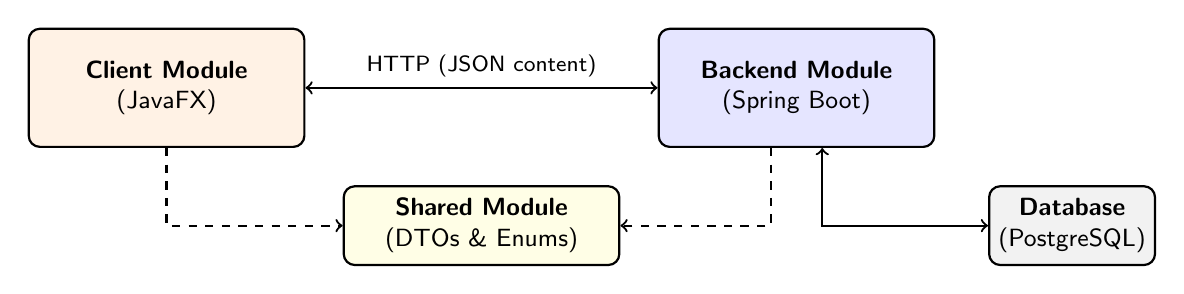
\begin{tikzpicture}[
    box/.style={draw=black, thick, rounded corners, minimum width=3.5cm, minimum height=1.5cm, align=center, fill=blue!5, font=\sffamily\small},
    dbbox/.style={draw=black, thick, rounded corners, minimum height=1.5cm, minimum width=2cm, fill=yellow!10, align=center, font=\sffamily\small},
    arrow/.style={->, thick},
    dasharrow/.style={->, dashed, thick}
]
    \node[box, fill=orange!10] (client) at (-4, 0) {\textbf{Client Module} \\ (JavaFX)};
    \node[box, fill=blue!10] (backend) at (4, 0) {\textbf{Backend Module} \\ (Spring Boot)};
    \node[box, minimum height=1cm, fill=yellow!10] (shared) at (0, -1.75) {\textbf{Shared Module} \\ (DTOs \& Enums)};
    \node[dbbox, minimum height=1cm, fill=gray!10] (db) at (7.5, -1.75) {\textbf{Database} \\ (PostgreSQL)};

    \draw[arrow, <->] (client) -- node[above, font=\footnotesize\sffamily] {HTTP (JSON content)} (backend);
    \draw[dasharrow] (client) |- (shared);
    \draw[dasharrow] ([xshift=-0.75cm] backend) |- (shared);
    \draw[arrow, <->] ([xshift=0.75cm] backend) |- (db);

\end{tikzpicture}
\caption{High-Level Modular Architecture}
\end{figure}

\section{Technological Stack}
The application leverages \textbf{Java 17+} and relies on the following core technologies to fulfill its functional and non-functional requirements:

\begin{itemize}
    \item \textbf{Server:} \textit{Spring Boot} provides the foundational inversion of control and auto-configuration. Routing is handled by \textit{Spring Web MVC}, while \textit{Spring Security} enforces JWT-based authentication. The data layer utilizes \textit{Spring Data JPA} and \textit{Hibernate} for Object-Relational Mapping (ORM) against a relational database (\textit{PostgreSQL} / \textit{H2} (for testing)).
    \item \textbf{Client:} \textit{JavaFX} serves as the framework for the Graphical User Interface.
    \item \textbf{Tooling:} \textit{Apache Maven} coordinates multi-module dependency management and the build lifecycle. \textit{JUnit 5} and \textit{Mockito} facilitate unit testing and test-driven development methodologies.
\end{itemize}

\section{Backend Architecture}
The server implements a strict 3-tier logical layered architecture, which separates concerns and isolates business logic from the network protocols.

\begin{enumerate}
    \item \textbf{Controller Layer:} Handles incoming HTTP connections, maps REST endpoints, and deserializes JSON requests. It delegates instructions to the underlying services, then serializes the results into a JSON response that gets sent back to the requesting client.
    \item \textbf{Service Layer:} This tier encapsulates the core business rules (e.g. debt reduction algorithms). It performs strict validation and defines transactional boundaries to guarantee data atomicity and avoid corruption.
    \item \textbf{Data Access Layer (Repository):} Contains Spring Data JPA interfaces that abstract raw SQL, handling complex queries that map database tables directly to standard Java Objects.
\end{enumerate}

\section{Client Architecture}
The client module implements an API-first architectural design. It mirrors the backend services via dedicated client-side classes injected with a centralized HTTP client wrapper. These classes build requests, include the session JWT in the \texttt{'Authorization: Bearer'} header and deserialize the JSON server responses. By wrapping the REST communication in these service classes, the JavaFX UI controllers remain completely unaware of the underlying network protocols, adhering strictly to the Single Responsibility Principle.

\section{Detailed Architecture Diagram}

\begin{figure}[H]
    \centering
    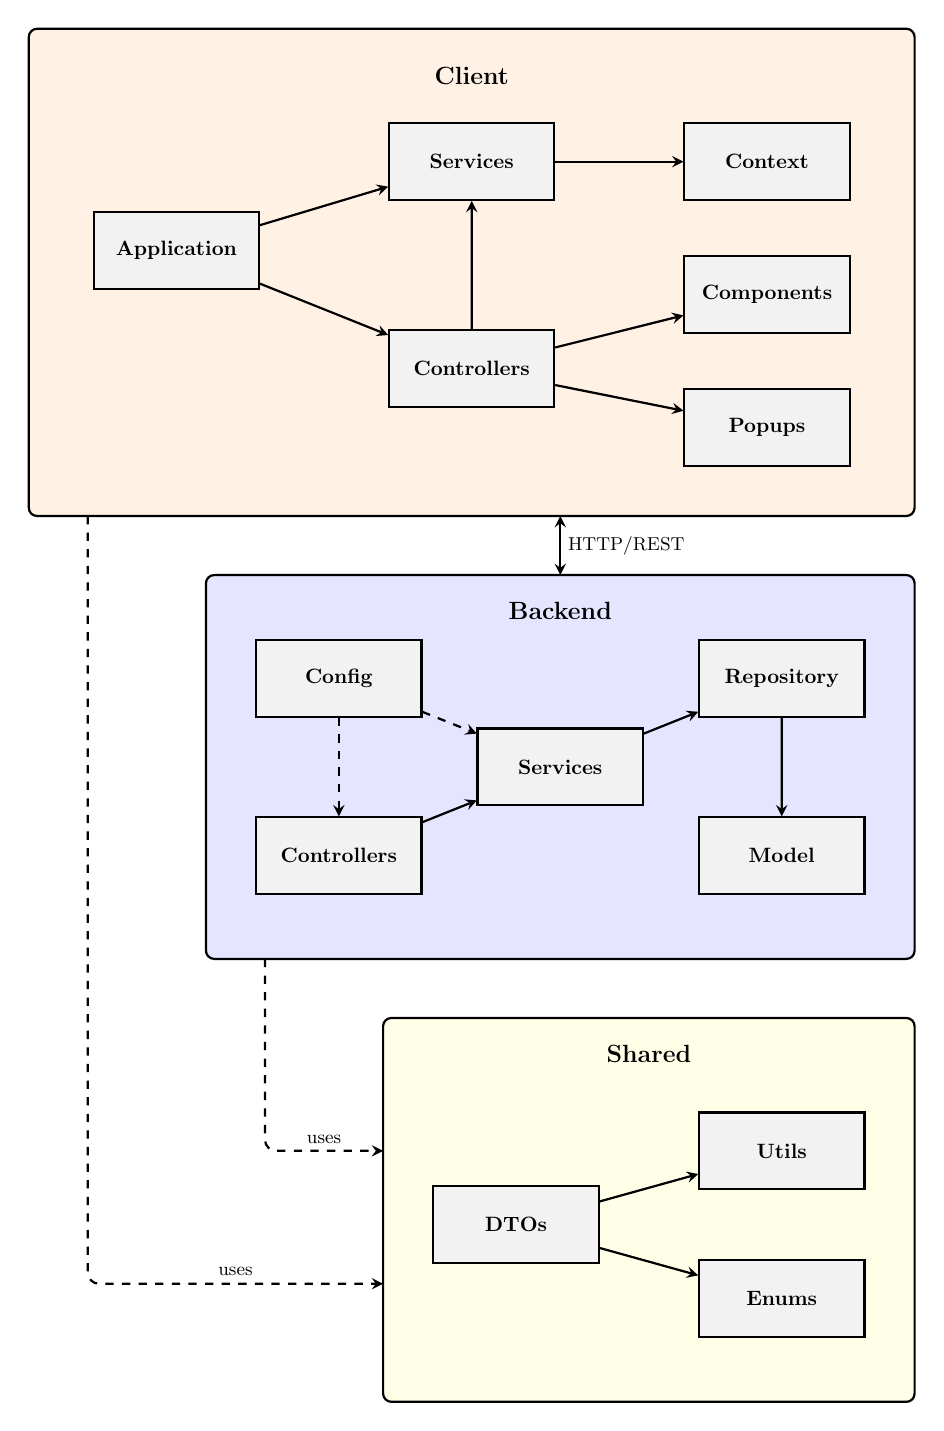
\begin{tikzpicture}[
        scale=0.75, transform shape, % <--- Adjust the 0.7 to change the overall size
        font=\sffamily,
        >=stealth,
        % Define the style for simple rectangles
        umlbox/.style={
            rectangle, draw, thick, fill=gray!10,
            minimum width=2.8cm, minimum height=1.3cm,
            align=center, font=\bfseries
        }
    ]
    
        % ==========================
        % BOUNDING BOXES (BACKGROUND)
        % ==========================
        % Client Box
        \draw[thick, fill=orange!10, rounded corners=3pt] (-5, 2.25) rectangle (10, -6);
        \node[font=\bfseries\large] at (2.5, 1.45) {\textbf{Client}};
    
        % Backend Box
        \draw[thick, fill=blue!10, rounded corners=3pt] (-2, -7) rectangle (10, -13.5);
        \node[font=\bfseries\large] at (4, -7.6) {\textbf{Backend}};
    
        % Shared Box
        \draw[thick, fill=yellow!10, rounded corners=3pt] (1, -14.5) rectangle (10, -21);
        \node[font=\bfseries\large] at (5.5, -15.1) {\textbf{Shared}};
    
    
        % ==========================
        % CLIENT NODES
        % ==========================
        % Neatly arranged in a 3-column grid within the client bounds
        \node[umlbox] (app)       at (-2.5, -1.5) {Application};
        \node[umlbox] (svcClient) at (2.5, 0)     {Services};
        \node[umlbox] (ctrl)      at (2.5, -3.5)    {Controllers};
        \node[umlbox] (ctx)       at (7.5, 0)     {Context};
        \node[umlbox] (comp)      at (7.5, -2.25)  {Components};
        \node[umlbox] (pop)       at (7.5, -4.5)  {Popups};
    
        % Client Connections
        \draw[->, thick] (app) -- (svcClient);
        \draw[->, thick] (app) -- (ctrl);
        \draw[->, thick] (ctrl) -- (svcClient);
        \draw[->, thick] (ctrl) -- (comp);
        \draw[->, thick] (ctrl) -- (pop);
        \draw[->, thick] (svcClient) -- (ctx);
    
    
        % ==========================
        % BACKEND NODES
        % ==========================
        % Arranged to flow from left to right within the backend bounds
        \node[umlbox] (config)      at (0.25, -8.75)  {Config};
        \node[umlbox] (ctrlBackend) at (0.25, -11.75) {Controllers};
        \node[umlbox] (svcBackend)  at (4, -10.25)   {Services};
        \node[umlbox] (repo)        at (7.75, -8.75)  {Repository};
        \node[umlbox] (model)       at (7.75, -11.75) {Model};
    
        % Backend Connections
        \draw[->, thick, dashed] (config) -- (svcBackend);
        \draw[->, thick, dashed] (config) -- (ctrlBackend);
        \draw[->, thick] (ctrlBackend) -- (svcBackend);
        \draw[->, thick] (svcBackend) -- (repo);
        \draw[->, thick] (repo) -- (model);
    
    
        % ==========================
        % SHARED NODES
        % ==========================
        % Centered hierarchically within the shared bounds
        \node[umlbox] (dto)   at (3.25, -18) {DTOs};
        \node[umlbox] (utils) at (7.75, -16.75)   {Utils};
        \node[umlbox] (enums) at (7.75, -19.25)   {Enums};
    
        % Shared Connections
        \draw[->, thick] (dto) -- (utils);
        \draw[->, thick] (dto) -- (enums);
    
    
        % ==========================
        % CROSS-BOUNDARY DEPENDENCIES
        % ==========================
        % Client -> Backend (HTTP/REST)
        \draw[<->, thick] (4, -6) -- 
            node[right, font=\small] {HTTP/REST} (4, -7);
    
        % Client -> Shared (uses)
        % Uses orthogonal routing ( |-) to bypass the backend box safely on the left
        \draw[->, thick, dashed, rounded corners] (-4, -6) |- 
            node[pos=0.75, above, font=\small] {uses} (1, -19);
    
        % Backend -> Shared (uses)
        \draw[->, thick, dashed, rounded corners] (-1, -13.5) |- 
            node[pos = 0.75, above, font=\small] {uses} (1, -16.75);
    
    \end{tikzpicture}
    \caption{Detailed architecture diagram}
    \label{fig:uml_overview}
\end{figure}

\section{Example: User Request Flow}

The following diagram illustrates the lifecycle of a user request, tracing its path through the architecture, its interaction with the database and the return of the response back to the user.

\begin{figure}[H]
\centering
\resizebox{\textwidth}{!}{%
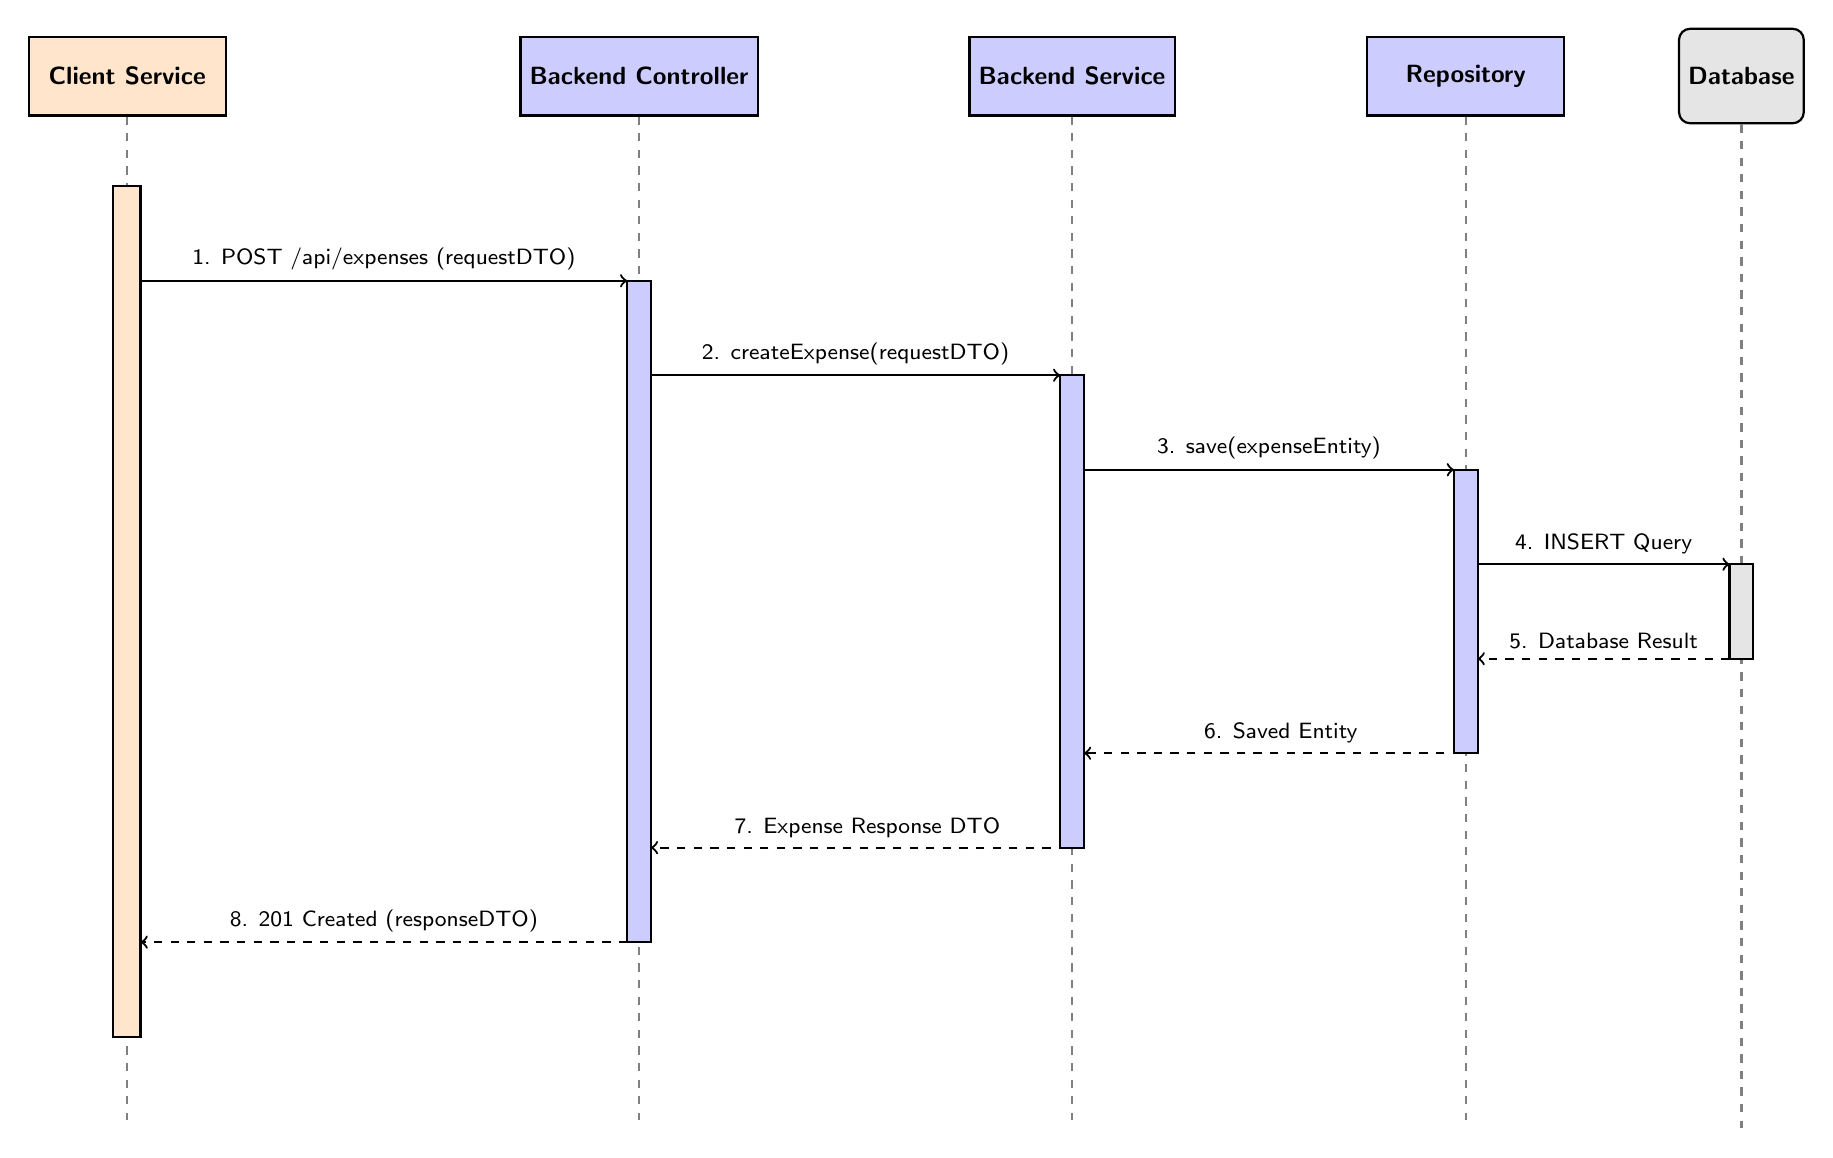
\begin{tikzpicture}[
    lifeline/.style={thick, dashed, draw=gray},
    box/.style={draw=black, thick, fill=blue!5, minimum width=2.5cm, minimum height=1cm, font=\sffamily\small\bfseries, align=center},
    dbbox/.style={draw=black, thick, rounded corners, minimum height=1.2cm, minimum width=1.5cm, fill=yellow!10, align=center, font=\sffamily\small\bfseries},
    msg/.style={->, thick, font=\footnotesize\sffamily},
    return/.style={->, dashed, thick, font=\footnotesize\sffamily}
]

% Nodes
\node[box, fill=orange!20] (client) at (-0.5, 1.6) {Client Service};
\node[box, fill=blue!20] (controller) at (6, 1.6) {Backend Controller};
\node[box, fill=blue!20] (service) at (11.5, 1.6) {Backend Service};
\node[box, fill=blue!20] (repository) at (16.5, 1.6) {Repository};
\node[dbbox, fill=gray!20] (db) at (20, 1.6) {Database};

% Lifelines
\draw[lifeline] (client.south) -- +(0, -12.75);
\draw[lifeline] (controller.south) -- +(0, -12.75);
\draw[lifeline] (service.south) -- +(0, -12.75);
\draw[lifeline] (repository.south) -- +(0, -12.75);
\draw[lifeline] (db.south) -- +(0, -12.75);

% UML Activation Boxes
\draw[fill=orange!20, draw=black, thick] (-0.68, 0.2) rectangle (-0.33, -10.6);   % Client
\draw[fill=blue!20, draw=black, thick] (5.85, -1) rectangle (6.15, -9.4);    % Controller
\draw[fill=blue!20, draw=black, thick] (11.35, -2.2) rectangle (11.65, -8.2);  % Service
\draw[fill=blue!20, draw=black, thick] (16.35, -3.4) rectangle (16.65, -7.0); % Repository
\draw[fill=gray!20, draw=black, thick] (19.85, -4.6) rectangle (20.15, -5.8); % DB

% Messages
\draw[msg] (-0.33, -1) -- node[above] {1. POST /api/expenses (requestDTO)} (5.85, -1);
\draw[msg] (6.15, -2.2) -- node[above] {2. createExpense(requestDTO)} (11.35, -2.2);
\draw[msg] (11.65, -3.4) -- node[above] {3. save(expenseEntity)} (16.35, -3.4);
\draw[msg] (16.65, -4.6) -- node[above] {4. INSERT Query} (19.85, -4.6);

\draw[return] (19.85, -5.8) -- node[above] {5. Database Result} (16.65, -5.8);
\draw[return] (16.65, -7.0) -- node[above] {6. Saved Entity} (11.65, -7.0);
\draw[return] (11.65, -8.2) -- node[above] {7. Expense Response DTO} (6.15, -8.2);
\draw[return] (5.85, -9.4) -- node[above] {8. 201 Created (responseDTO)} (-0.33, -9.4);

\end{tikzpicture}}%
\caption{User request flow: Adding an Expense}
\end{figure}

\chapter{API Documentation}
\section{RESTful APIs}
The server interacts with the client purely through HTTP protocols. The API design adheres strictly to standard RESTful architectures mapping HTTP verbs directly to CRUD operations on underlying resources.

\section{General Rules and Detailed Endpoints Description}
The entire API layer of the application has been developed using two fundamental rules, to ensure coherence, avoidance of code repetition and backend data protection:
\begin{itemize}
    \item Every endpoint which requires information about the account the requesting client is logged in as receives such information through the \texttt{@AuthenticationPrincipal UserDetails userDetails} construct, to safely use the JWT token each request must include in its headers and prevent data leaks.
    \item In the description of each endpoint, the \texttt{/\{<id>\}} construct implies that the Controller method requires an additional parameter (the UUID of an object to perform some operation on it) and that it declares that parameter as a \texttt{@PathVariable UUID <id>}.
\end{itemize}
A detailed description of all the endpoints exposed by the application's backend, grouped by the Controller class they belong to, follows next.

\subsection{Authentication Controller (\texttt{/api/auth})}
This module allows for anonymous operations to establish session credentials.
\begin{itemize}
    \item \textbf{POST /register:} Accepts user registration details. Returns standard 201 Created on success.
    \item \textbf{POST /login:} Authenticates user. Returns JWT payload upon HTTP 200 OK.
\end{itemize}

\subsection{Household Controller (\texttt{/api/household})}
Manages generic grouping of users.
\begin{itemize}
    \item \textbf{POST /create:} Instantiates a generic household container.
    \item \textbf{POST /join:} Registers the current user token against an existing household grouping.
    \item \textbf{GET /\{id\}}: Retrieves details about a specific household, ensuring the requester has valid authorizations.
\end{itemize}

\subsection{User Controller (\texttt{/api/users})}
\begin{itemize}
    \item \textbf{GET /me:}
\end{itemize}

\subsection{Expense Management Controllers}
The financial subsystem of the application is decomposed into three separate controllers, each responsible for a distinct concern: expense recording, debt tracking, and settlement processing. All endpoints within this subsystem retrieve the requesting user's identity from the JWT token, and use it to resolve the user's current household, ensuring strict data isolation between households.

\subsubsection{Expense Controller (\texttt{/api/expenses})}
Handles the creation and retrieval of shared expenses within a household.
\begin{itemize}
    \item \textbf{POST:} Receives an \texttt{ExpenseCreateRequestDTO} payload containing a description, a total monetary amount, a split type (one of the \texttt{ExpenseSplitType} enumeration values: \texttt{EQUAL\_SPLIT}, \texttt{SHARES}, \texttt{EXACT\_AMOUNT}, or \texttt{ADJUSTMENT}), and a list of \texttt{ExpenseShareRequestDTO} entries, each specifying a user UUID and, depending on the split type, an additional value (such as the exact amount or number of shares). The requesting user is automatically recorded as the payer. Upon successful creation the endpoint returns an \texttt{ExpenseResponseDTO}, containing the persisted expense's UUID, description, timestamp, total amount, payer information, split type, household identifier, and the computed list of individual shares, with HTTP status 201 Created.

    \item \textbf{GET:} Retrieves a filtered list of expenses for the requesting user's household. Filter criteria are supplied as query parameters through a \texttt{TransactionFilterRequestDTO}, which supports the following optional filters: \texttt{householdId} (UUID), \texttt{userTransactionRole} (one of \texttt{CREDITOR}, \texttt{DEBTOR}, or \texttt{ALL}, to select expenses where the user is the payer, a participant, or either), \texttt{dateRange} (a date interval), and \texttt{description} (a textual search term). Returns a list of \texttt{ExpenseResponseDTO} objects with HTTP status 200 OK.

    \item \textbf{GET /overview:} Returns an \texttt{ExpenseOverviewResponseDTO} containing aggregated statistics for the current calendar month within the requesting user's household: the total amount across all expenses and the count of expenses recorded. Returns HTTP status 200 OK.

    \item \textbf{GET /me:} Returns a \texttt{UserNetOverviewResponseDTO} containing a single \texttt{actualCashFlowAmount} value representing the requesting user's net financial position for the current month. A positive value indicates the user has paid more than they had to (other members owe the user money), while a negative value indicates the opposite. Returns HTTP status 200 OK.
\end{itemize}

\subsubsection{Debt Controller (\texttt{/api/debts})}
Manages the retrieval and deletion of individual debt records. Debts are automatically generated by the backend whenever a new expense is created: the system computes each participant's owed share and persists directed debt edges between the payer (creditor) and each owing participant (debtor).
\begin{itemize}
    \item \textbf{GET:} Retrieves a filtered list of debt records for the requesting user's household. Filter criteria are supplied as query parameters through a \texttt{DebtFilterRequestDTO}, which requires a mandatory \texttt{userTransactionRole} parameter (one of \texttt{CREDITOR}, \texttt{DEBTOR}, or \texttt{ALL}) to select debts where the requesting user is owed money, owes money, or either. An optional \texttt{involvedId} parameter (UUID) can further narrow results to debts involving a specific counterpart. Each returned \texttt{DebtResponseDTO} contains the debt's UUID, the requesting user's transaction role, the involved counterpart's UUID and full name, and the outstanding monetary amount. Returns HTTP status 200 OK.

    \item \textbf{GET /me:} Returns a \texttt{DebtOverviewResponseDTO} summarising the requesting user's aggregate debt position: \texttt{totalOwedByMe} (the sum of all debts where the user is the debtor) and \texttt{totalOwedToMe} (the sum of all debts where the user is the creditor). Returns HTTP status 200 OK.

    \item \textbf{DELETE /\{debtId\}:} Deletes the debt record identified by \texttt{debtId}. Returns HTTP status 204 No Content upon successful deletion.
\end{itemize}

\subsubsection{Settlement Controller (\texttt{/api/settlements})}
Handles the creation and retrieval of settlement transactions. A settlement represents a real-world payment made by a debtor to a creditor to reduce or eliminate an unpaid debt.
\begin{itemize}
    \item \textbf{POST /\{debtId\}:} Creates a new settlement against the debt identified by the path variable \texttt{debtId}. The request body is a \texttt{SettlementCreateRequestDTO} containing the target \texttt{debtId}, the \texttt{creditorId} (UUID of the user receiving the payment), the settlement \texttt{amount} (which must be strictly positive), and an optional textual \texttt{description}. The backend reduces the referenced debt's balance by the settlement amount. Returns the persisted \texttt{SettlementResponseDTO} containing the settlement's UUID, the requesting user's transaction role, the involved counterpart's UUID and full name, the settled amount, timestamp, description, and household identifier, with HTTP status 201 Created.

    \item \textbf{GET:} Retrieves a filtered list of settlement records for the requesting user's household. Filter criteria are supplied as query parameters through a \texttt{TransactionFilterRequestDTO} (the same filter object used by the Expense Controller's GET endpoint), supporting optional filters for \texttt{householdId}, \texttt{userTransactionRole}, \texttt{dateRange}, and \texttt{description}. Returns a list of \texttt{SettlementResponseDTO} objects with HTTP status 200 OK.
\end{itemize}

\subsection{Chore Controller (\texttt{/api/chores})}
Handles chores and chore assignments related operations. All of the following endpoints retrieve the requesting user's information, to ensure that every user is only allowed to access chores and assignments related to it or its household, and to block admin-only actions to unauthorized users 
\begin{itemize}
    \item \textbf{POST:} Receives a \texttt{ChoreCreateRequestDTO} payload to create a new chore. 
    \item \textbf{POST /assignments:} Receives a \texttt{ChoreAssignmentCreateRequestDTO} payload to create a new chore assignment.
    \item \textbf{GET:} Returns all chores, as \texttt{ChoreResponseDTO}, of the requesting user's current household.
    \item \textbf{GET /assignments:} Returns chore assignments, as \texttt{ChoreAssignmentResponseDTO}, based on the filters provided by the \texttt{ChoreAssignmentFilterRequestDTO} payload.
    \item \textbf{GET /assignments/me:} Returns an \texttt{AssignmentOverviewDTO} with the total counts of pending and overdue assignments of the requesting user
    \item \textbf{GET /assignments/overview:} Returns an \texttt{AssignmentOverviewDTO} with the total counts of pending and overdue assignments of the requesting user's current household
    \item \textbf{PATCH /assignments/\{assignmentId\}/status:} Receives a \texttt{ChoreStatusUpdateRequestDTO} payload to find the chore assignment identified by \texttt{assignmentId} and update its status
    \item \textbf{DELETE /\{choreId\}:} Deletes the chore identified by \texttt{choreId}. Admin-only action 
    \item \textbf{DELETE /assignments/\{assignmentId\}:} Deletes the chore assignment identified by \texttt{assignmentId}. Admin-only action.
\end{itemize}

\subsection{Shopping List Controller (\texttt{/api/shopping-lists})}
\begin{itemize}
    \item \textbf{POST: } Receives a \texttt{ShoppingListCreateRequestDTO} payload to create a new shopping list, and returns 201 OK with a \texttt{ShoppingListResponseDTO}
    \item \textbf{GET: } Returns all the shopping lists, as \texttt{ShoppingListResponseDTO}, of the requesting user's current household
    \item \textbf{PATCH /\{listId\}:} Receives a \texttt{ShoppingListUpdateRequestDTO} payload to update the status of an existing list (identified by \texttt{listId}), which simply consists of a list of booleans used to update the \texttt{isBought} attribute for each item in the list.
    \item \textbf{DELETE/\{listId\}:} Deletes an existing shopping list (identified by \texttt{listId}).
\end{itemize}

% TO DO (For 60-page target): 
% Include massive swagger/OpenAPI spec screenshots or table dumps. Document EVERY SINGLE API endpoint your application provides. For each endpoint, show the exact JSON request payload object and exact JSON response object. 
% Example:
% \subsubsection{Endpoint: Create Chore}
% \textbf{URL:} \texttt{/api/chores} \\
% \textbf{Method:} \texttt{POST} \\
% \textbf{Request Body:} 
% \begin{lstlisting}[language=json]
% { "title": "Take out trash", "assignedTo": 12, "dueDate": "2026-05-05" }
% \end{lstlisting}
% You must expand this structure out for all controller definitions to fulfill thorough API documentation paradigms.

\chapter{Backend Design and Implementation}

\section{Domain Model Design}
The application fundamentally requires a robust, scalable, and normalized relational database schema to model the physical reality of shared households. The detailed design of these models forms the crux of the backend entity schemas.

\subsection{Core Entities mapping}
The core system entities residing in the \texttt{model} package are designed based on precise relational mappings:

\begin{itemize}
    \item \textbf{User:} Represents an individual utilizing the application. Has an ID, credential mappings, and profile information.
    \item \textbf{Household:} The central grouping object. A generic \texttt{Household} has a one-to-many relationship mapping users interacting within it.
    \item \textbf{Expense:} Represents a shared financial transaction logged within a household. Stores the total amount, a textual description, the payer reference, the household it belongs to, and the split type used to divide the cost. The timestamp is set automatically at creation time. An Expense owns a one-to-many collection of \texttt{ExpenseShare} children with \texttt{CascadeType.ALL} and \texttt{orphanRemoval = true}, so persisting the parent automatically persists all of its shares in a single transactional write.
    \item \textbf{ExpenseShare:} Represents a single user's computed portion of an Expense. Each record links back to the parent Expense and to the involved User, and stores the monetary amount that user owes. Share amounts are always strictly positive; users with a zero contribution are excluded from the share list entirely.
    \item \textbf{Settlement:} Records a real-world payment made by a debtor to a creditor to reduce an outstanding debt. Each Settlement references the Debt it applies to, the two involved users, the amount paid, an optional description, and a timestamp. The household identifier is denormalized from the parent Debt into the Settlement entity to enable efficient household-scoped queries without requiring a join through the Debt table.
    \item \textbf{Debt:} Models a directed financial obligation between two users within a household: one debtor who owes money and one creditor who is owed. Its amount can be increased by new expenses and decreased by settlements or by the automatic netting logic. Crucially, a fully settled Debt is never deleted: its amount is set to zero and the record is preserved (see Section~\ref{sec:debt-lifecycle}).
    \item \textbf{Chore / ChoreAssignment:} A task representation and the mapping connecting the task to specific user timelines.
\end{itemize}

\subsection{Complete Database ER Diagram}


%ER diagram figure
\begin{figure}[H]
\makebox[\textwidth][c]{% Centers the oversized diagram on the page

\resizebox{1,1\textwidth}{!}{

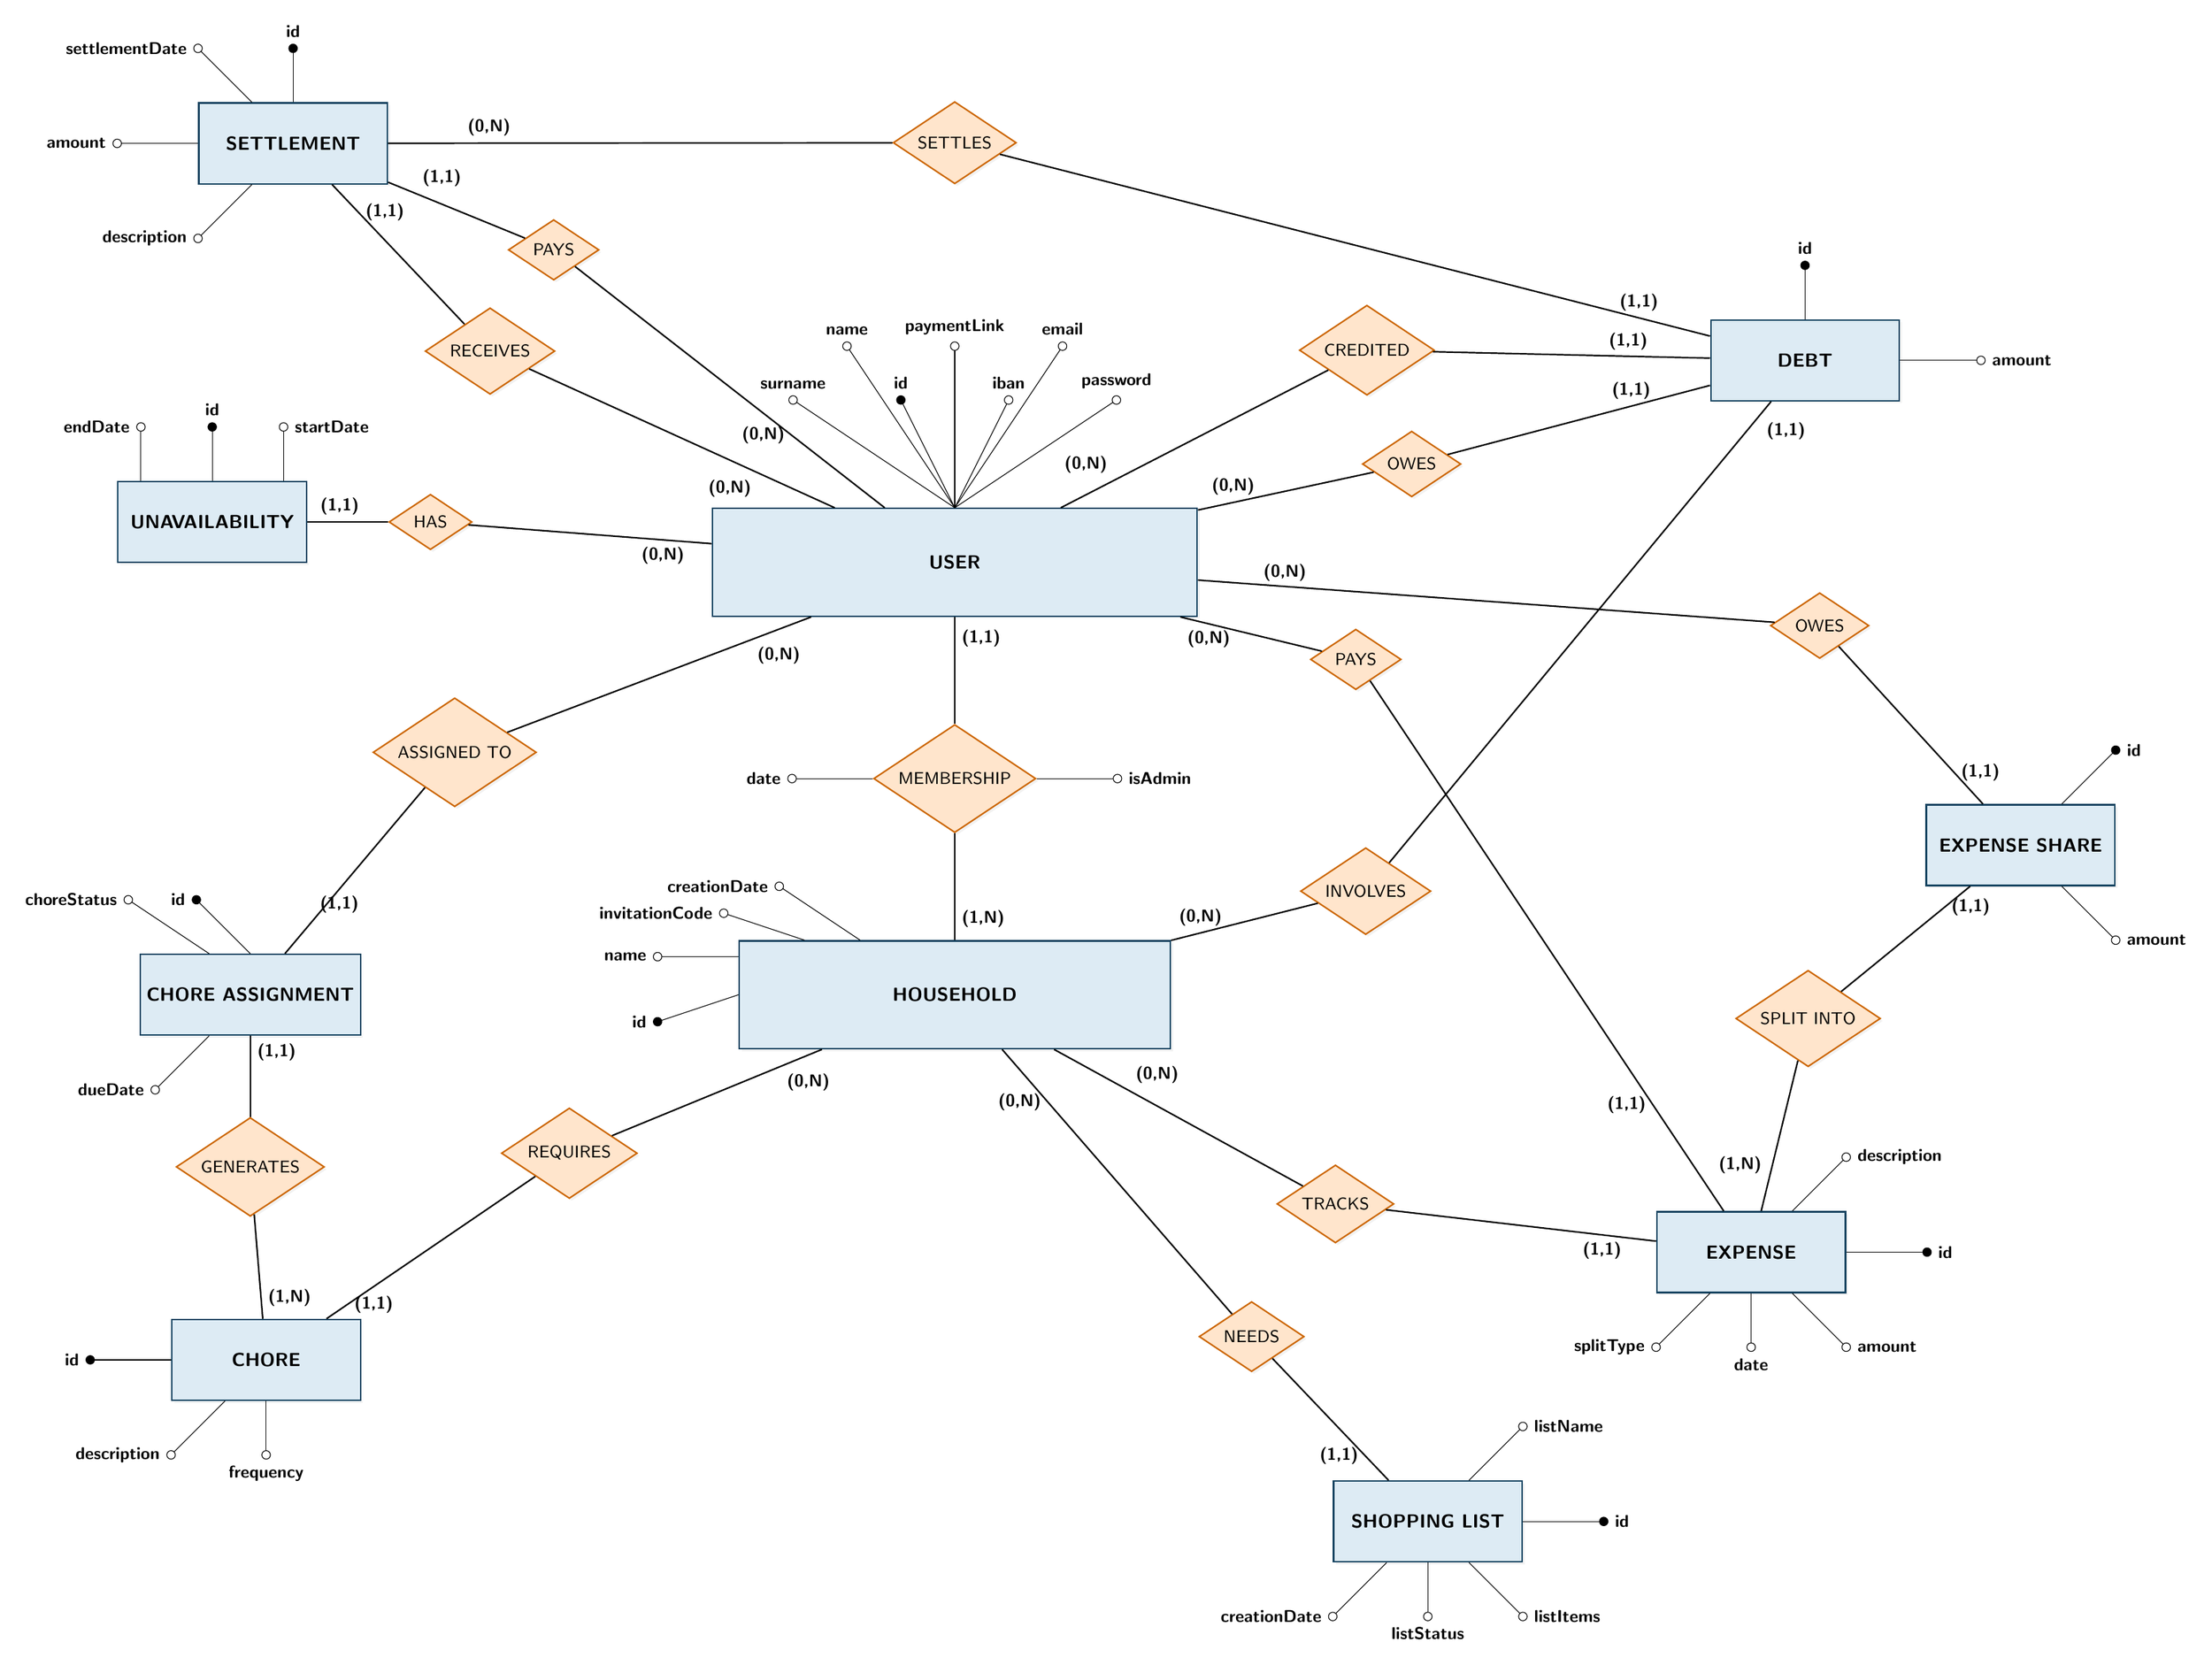
\begin{tikzpicture}[
    % --- STILI GLOBALI DEL DIAGRAMMA ---
    node distance = 1.5cm and 3cm,
    entity/.style={
        rectangle,
        fill=UMLBlue!40, 
        draw=UMLDarkBlue,
        line width=0.8pt,
        minimum width=3.5cm,
        minimum height=1.5cm,
        align=center,
        font=\sffamily\bfseries,
        drop shadow={opacity=0.1, shadow xshift=0.3ex, shadow yshift=-0.3ex}
    },
    relationship/.style={
        diamond,
        fill=orange!20,
        draw=orange!80!black,
        line width=0.8pt,
        aspect=1.5,
        align=center,
        font=\small\sffamily,
        drop shadow={opacity=0.1, shadow xshift=0.3ex, shadow yshift=-0.3ex}
    },
    pk/.style={ % Stile per Chiave Primaria (Pallino nero)
        circle,
        fill=black,
        draw=black,
        inner sep=0pt,
        minimum size=4.5pt
    },
    attr/.style={ % Stile per Attributo Normale (Pallino bianco)
        circle,
        fill=white,
        draw=black,
        inner sep=0pt,
        minimum size=4.5pt
    },
    lbl/.style={
        font=\small\sffamily\bfseries
    }
]

  % ==========================================
  % 1. ENTITIES
  % ==========================================
  
  % Central Anchor
  \node[entity, minimum width=8cm, minimum height=2cm] (household) {HOUSEHOLD};

  % User at the top
  \node[entity, minimum width=9cm, minimum height=2cm] (user) [above=6cm of household] {USER};
  \node[entity] (settlement) [above left=6cm and 6cm of user] {SETTLEMENT};

  % Entities relative to Household
  \node[entity] (expense) [below right=3cm and 9cm of household] {EXPENSE};
  \node[entity] (shopping_list) [below right=8cm and 3cm of household] {SHOPPING LIST};
  \node[entity] (expense_share) [above right=1cm and 14cm of household] {EXPENSE SHARE};
  \node[entity] (debt) [above right=10cm and 10cm of household] {DEBT};
  \node[entity] (unavailability) [above left=7cm and 8cm of household] {UNAVAILABILITY};
  \node[entity] (chore) [below left=5cm and 7cm of household] {CHORE};
  \node[entity] (chore_assignment) [left=7cm of household] {CHORE ASSIGNMENT};

% ==========================================
  % 2. ATTRIBUTES (New stalk-and-circle style)
  % ==========================================

  % USER Attributes (Squeezed to the top center to avoid corner links)
  \draw (user.90) -- ++(3, 2) node[attr, label={[lbl]above:password}] {};
  \draw (user.90) -- ++(2, 3) node[attr, label={[lbl]above:email}] {};
  \draw (user.90)  -- ++(1, 2) node[attr, label={[lbl]above:iban}] {};
  \draw (user.90)  -- ++(0, 3)    node[attr, label={[lbl]above:paymentLink}] {};
  \draw (user.90)  -- ++(-1, 2)  node[pk, label={[lbl]above:id}] {};
  \draw (user.90)  -- ++(-2, 3)  node[attr, label={[lbl]above:name}] {};
  \draw (user.90) -- ++(-3, 2)  node[attr,   label={[lbl]above:surname}] {};

  % UNAVAILABILITY Attributes
  \draw (unavailability.90)  -- ++(0,1)    node[pk,   label={[lbl]above:id}] {};
  \draw (unavailability.30)  -- ++(0,1)    node[attr, label={[lbl]right:startDate}] {};
  \draw (unavailability.150) -- ++(0,1)    node[attr, label={[lbl]left:endDate}] {};

  % HOUSEHOLD Attributes (Shifted away from the bottom-left corner to avoid REQUIRES)
  \draw (household.180) -- ++(-1.5,-0.5) node[pk,   label={[lbl]left:id}] {};
  \draw (household.170) -- ++(-1.5,0)    node[attr, label={[lbl]left:name}] {};
  \draw (household.160) -- ++(-1.5,0.5)  node[attr, label={[lbl]left:invitationCode}] {};
  \draw (household.150) -- ++(-1.5,1.0)  node[attr, label={[lbl]left:creationDate}] {};

  % SHOPPING LIST Attributes
  \draw (shopping_list.0)   -- ++(1.5,0)   node[pk,   label={[lbl]right:id}] {};
  \draw (shopping_list.45)  -- ++(1,1)     node[attr, label={[lbl]right:listName}] {};
  \draw (shopping_list.315) -- ++(1,-1)    node[attr, label={[lbl]right:listItems}] {};
  \draw (shopping_list.270) -- ++(0,-1)    node[attr, label={[lbl]below:listStatus}] {};
  \draw (shopping_list.225) -- ++(-1,-1)   node[attr, label={[lbl]left:creationDate}] {};

  % EXPENSE Attributes
  \draw (expense.0)   -- ++(1.5,0)  node[pk,   label={[lbl]right:id}] {};
  \draw (expense.45)  -- ++(1,1)    node[attr, label={[lbl]right:description}] {};
  \draw (expense.315) -- ++(1,-1)   node[attr, label={[lbl]right:amount}] {};
  \draw (expense.270) -- ++(0,-1)   node[attr, label={[lbl]below:date}] {};
  \draw (expense.225) -- ++(-1,-1)  node[attr, label={[lbl]left:splitType}] {};

  % EXPENSE SHARE Attributes
  \draw (expense_share.45)  -- ++(1,1)   node[pk,   label={[lbl]right:id}] {};
  \draw (expense_share.315) -- ++(1,-1)  node[attr, label={[lbl]right:amount}] {};

  % DEBT Attributes
  \draw (debt.90) -- ++(0,1)   node[pk,   label={[lbl]above:id}] {};
  \draw (debt.0)  -- ++(1.5,0) node[attr, label={[lbl]right:amount}] {};

  % SETTLEMENT Attributes
  \draw (settlement.90)  -- ++(0,1)    node[pk,   label={[lbl]above:id}] {};
  \draw (settlement.180) -- ++(-1.5,0) node[attr, label={[lbl]left:amount}] {};
  \draw (settlement.135) -- ++(-1,1)   node[attr, label={[lbl]left:settlementDate}] {};
  \draw (settlement.225) -- ++(-1,-1)  node[attr, label={[lbl]left:description}] {};

  % CHORE Attributes
  \draw (chore.180) -- ++(-1.5,0)  node[pk,   label={[lbl]left:id}] {};
  \draw (chore.225) -- ++(-1,-1)   node[attr, label={[lbl]left:description}] {};
  \draw (chore.270) -- ++(0,-1)    node[attr, label={[lbl]below:frequency}] {};

  % CHORE ASSIGNMENT Attributes
  \draw (chore_assignment.90) -- ++(-1,1)   node[pk,   label={[lbl]left:id}] {};
  \draw (chore_assignment.135) -- ++(-1.5,1) node[attr, label={[lbl]left:choreStatus}] {};
  \draw (chore_assignment.225) -- ++(-1,-1)  node[attr, label={[lbl]left:dueDate}] {};

  % ==========================================
  % 3. RELATIONSHIP DIAMONDS & ATTRIBUTES
  % ==========================================

% MEMBERSHIP (Centered between User and Household)
  \node[relationship] (membership) at ($(user)!0.5!(household)$) {MEMBERSHIP};
  \draw (membership.0)   -- ++(1.5,0)  node[attr, label={[lbl]right:isAdmin}] {};
  \draw (membership.180) -- ++(-1.5,0) node[attr, label={[lbl]left:date}] {};

  % HAS (User <-> Unavailability)
  \node[relationship] (has_unav) [right=1.5cm of unavailability] {HAS};

  % SETTLEMENT <-> USER (PAYS and RECEIVES)
  \node[relationship] (pays_settle) [above left=4.5cm and 2.5cm of user] {PAYS};
  \node[relationship] (receives_settle) [above left=2.5cm and 3.5cm of user] {RECEIVES};

  % SETTLES (Settlement <-> Debt)
  \node[relationship] (settles_debt) [above=6cm of user] {SETTLES};

  % DEBT <-> USER (CREDITED and OWES)
  \node[relationship] (credited_debt) [above right=2.5cm and 2.5cm of user] {CREDITED};
  \node[relationship] (owes_debt) [above right=0.5 cm and 3 .5cm of user] {OWES};

  % INVOLVES (Household <-> Debt)
  \node[relationship] (house_debt) [above right=0.5cm and 3cm of household] {INVOLVES};

  % PAYS (User <-> Expense)
  \node[relationship] (pays_exp) [below right=0.5cm and 2.5cm of user] {PAYS};

  % EXPENSE SHARE Relationships
  \node[relationship] (owes_share) [above left=3cm and 1.5cm of expense_share] {OWES};
  \node[relationship] (split_into) [below left=2cm and 1.5cm of expense_share] {SPLIT INTO};

  % TRACKS (Household <-> Expense)
  \node[relationship] (house_exp) [below right=2.5cm and 2.5cm of household] {TRACKS};

  % NEEDS (Household <-> Shopping List)
  \node[relationship] (needs_list) [below right=5cm and 1cm of household] {NEEDS};

  % REQUIRES (Household <-> Chore)
  \node[relationship] (has_chore) [below left=1.5cm and 2.5cm of household] {REQUIRES};

  % GENERATES (Chore <-> Chore Assignment)
  \node[relationship] (generates_assign) [below=1.5cm of chore_assignment] {GENERATES};

  % ASSIGNED TO (User <-> Chore Assignment)
  \node[relationship] (assigned_to) [below left=2cm and 4cm of user] {ASSIGNED TO};

  % ==========================================
  % 4. LINKS AND CARDINALITIES (Min, Max)
  % ==========================================

  % MEMBERSHIP 
  \draw[thick] (user) -- node[lbl, right, pos=0.2] {(1,1)} (membership);
  \draw[thick] (household) -- node[lbl, right, pos=0.2] {(1,N)} (membership);

  % UNAVAILABILITY
  \draw[thick] (user) -- node[lbl, below, pos=0.2] {(0,N)} (has_unav);
  \draw[thick] (unavailability) -- node[lbl, above, pos=0.4] {(1,1)} (has_unav);

  % SETTLEMENT (User pays/receives, Debt settles)
  \draw[thick] (user) -- node[lbl, left, pos=0.3] {(0,N)} (pays_settle);
  \draw[thick] (settlement) -- node[lbl, above right, pos=0.2] {(1,1)} (pays_settle);
  
  \draw[thick] (user) -- node[lbl, below left, pos=0.25] {(0,N)} (receives_settle);
  \draw[thick] (settlement) -- node[lbl, right, pos=0.2] {(1,1)} (receives_settle);
  
  \draw[thick] (settlement) -- node[lbl, above, pos=0.2] {(0,N)} (settles_debt);
  \draw[thick] (debt) -- node[lbl, above, pos=0.1] {(1,1)} (settles_debt);

  % DEBT (Household involves, User is credited/owes)
  \draw[thick] (user) -- node[lbl, above left, pos=0.2] {(0,N)} (credited_debt);
  \draw[thick] (debt) -- node[lbl, above left, pos=0.2] {(1,1)} (credited_debt);
  
  \draw[thick] (user) -- node[lbl, above, pos=0.2] {(0,N)} (owes_debt);
  \draw[thick] (debt) -- node[lbl, above, pos=0.3] {(1,1)} (owes_debt);
  
  \draw[thick] (household) -- node[lbl, above, pos=0.2] {(0,N)} (house_debt);
  \draw[thick] (debt) -- node[lbl, below right, pos=0.03] {(1,1)} (house_debt);

  % EXPENSE (Household tracks, User pays)
  \draw[thick] (user) -- node[lbl, below, pos=0.2] {(0,N)} (pays_exp);
  \draw[thick] (expense) -- node[lbl, left, pos=0.2] {(1,1)} (pays_exp);
  
  \draw[thick] (household) -- node[lbl, above right, pos=0.3] {(0,N)} (house_exp);
  \draw[thick] (expense) -- node[lbl, below, pos=0.2] {(1,1)} (house_exp);

  % EXPENSE SHARE
  \draw[thick] (expense) -- node[lbl, above left, pos=0.2] {(1,N)} (split_into);
  \draw[thick] (expense_share) -- node[lbl, right, pos=0.2] {(1,1)} (split_into);
  
  \draw[thick] (user) -- node[lbl, above left, pos=0.2] {(0,N)} (owes_share);
  \draw[thick] (expense_share) -- node[lbl, right, pos=0.2] {(1,1)} (owes_share);

  % SHOPPING LIST
  \draw[thick] (household) -- node[lbl, left, pos=0.2] {(0,N)} (needs_list);
  \draw[thick] (shopping_list) -- node[lbl, left, pos=0.2] {(1,1)} (needs_list);

  % CHORE & CHORE ASSIGNMENT
  \draw[thick] (household) -- node[lbl, below right, pos=0.2] {(0,N)} (has_chore);
  \draw[thick] (chore) -- node[lbl, right, pos=0.1] {(1,1)} (has_chore);
  
  \draw[thick] (chore) -- node[lbl, right, pos=0.2] {(1,N)} (generates_assign);
  \draw[thick] (chore_assignment) -- node[lbl, right, pos=0.2] {(1,1)} (generates_assign);
  
  \draw[thick] (user) -- node[lbl, below right, pos=0.2] {(0,N)} (assigned_to);
  \draw[thick] (chore_assignment) -- node[lbl, above right, pos=0.2] {(1,1)} (assigned_to);
\end{tikzpicture}
}
}
\caption{Database ER Diagram}
\end{figure}

\section{Business Logic Design}

\section{Security Implementation}

Security is fundamentally handled via stateless JSON Web Tokens (JWT). When a user successfully authenticates against the \texttt{AuthController}, the system signs a JWT utilizing HMACA-SHA256 signature algorithms. This token is securely issued to the client.

\subsection{Authentication Filter Lifecycle}
To intercept incoming generic requests requesting protected resources (such as fetching a Household list), the system registers the \texttt{JwtAuthenticationFilter}.

\begin{lstlisting}[language=Java, caption=Abstract Representation of the JWT Validation Lifecycle]
public class JwtAuthenticationFilter extends OncePerRequestFilter {
    @Override
    protected void doFilterInternal(HttpServletRequest request, ...) {
        final String authHeader = request.getHeader("Authorization");
        if (authHeader == null || !authHeader.startsWith("Bearer ")) {
            filterChain.doFilter(request, response);
            return;
        }
        
        final String jwt = authHeader.substring(7);
        final String userEmail = jwtService.extractUsername(jwt);
        
        // Validation logic handling...
        if (jwtService.isTokenValid(jwt, userDetails)) {
            UsernamePasswordAuthenticationToken authToken = new UsernamePasswordAuthenticationToken(...);
            SecurityContextHolder.getContext().setAuthentication(authToken);
        }
        filterChain.doFilter(request, response);
    }
}
\end{lstlisting}

This prevents unauthenticated actors from invoking core APIs.

\section{Core Business Logic: Expense Management}
The financial subsystem of the application encompasses expense recording, debt tracking, settlement processing, and aggregated overview computation. All write operations are wrapped in Spring \texttt{@Transactional} boundaries to guarantee Atomicity, Consistency, Isolation, and Durability (ACID properties): if any step within a transaction fails, the entire operation is rolled back, preventing inconsistent or partial state from reaching the database.

\subsection{Expense Creation Flow}
The creation of an expense is the most complex transactional operation in the system, as it must atomically perform three distinct tasks: persist the expense record itself, compute and store each user's individual share, and update all affected debt balances.

When the \texttt{ExpenseService.createExpense} method is invoked, the following steps execute within a single database transaction:
\begin{enumerate}
    \item The requesting user (payer) and their current household are resolved from the database. If the user is not a member of any household, the operation is rejected immediately.
    \item A root \texttt{Expense} entity is initialized with the provided description, total amount, payer reference, household, and split type. Thanks to JPA's \texttt{CascadeType.ALL} on the Expense--ExpenseShare relationship, the parent and all its children will be persisted together in a single \texttt{save} call.
    \item The appropriate split calculation strategy is obtained from the \texttt{ExpenseSplitStrategyFactory} (discussed in Section~\ref{sec:strategy-pattern}) and invoked to produce a map of user UUIDs to computed monetary amounts.
    \item For each entry in the computed map, an \texttt{ExpenseShare} child entity is created and added to the parent's collection.
    \item The expense graph (parent and all shares) is persisted via \texttt{expenseRepository.save}.
    \item For every share whose user differs from the payer, the \texttt{DebtService.addDebt} method is called to update the debt ledger (discussed in Section~\ref{sec:debt-lifecycle}). The payer is excluded because a user cannot owe money to themselves.
\end{enumerate}
If any step fails---for example, a user UUID in the share list does not exist, or the split strategy detects an invalid configuration---the \texttt{@Transactional} annotation ensures Spring Data immediately rolls back the entire operation, preventing ``ghost'' expenses or orphaned share records from reaching the database.

\subsection{The Strategy Pattern for Expense Splitting}
\label{sec:strategy-pattern}
The computation of individual shares is decoupled from the expense creation logic through the Strategy design pattern. The \texttt{ExpenseService} acts as the \textit{Context} and delegates the share computation to the \texttt{ExpenseSplitStrategy} interface, which is implemented by four concrete strategies.

\begin{figure}[H]
\centering
% \resizebox is still used to guarantee it fits the margins, 
% but the relative positioning inside prevents aggressive shrinking.
\resizebox{\textwidth}{!}{%
\begin{tikzpicture}[
    % Added the positioning library
    node distance=1.5cm and 0.3cm,
    class/.style={
        rectangle, draw=black, fill=gray!10,
        minimum width=4cm, minimum height=1cm, % slightly reduced width
        align=center, font=\small\ttfamily
    },
    interface/.style={
        rectangle, draw=black, fill=gray!10,
        minimum width=4cm, minimum height=1cm,
        align=center, font=\small\ttfamily
    },
    impl/.style={->, dashed, thick},
    uses/.style={->, thick}
]

% 1. Interface (Center anchor point)
\node[interface] (strategy) {
    \guillemotleft interface\guillemotright \\
    \textbf{ExpenseSplitStrategy} \\
    \footnotesize + calculateShares(...)
};

% 2. Context (Positioned relative to the interface)
\node[class, left=1.5cm of strategy] (context) {
    \textbf{ExpenseService} \\
    \footnotesize (Context)
};

% 3. Concrete strategies (Positioned in a row below the interface)
\node[class, below left=1.5cm and 0.1cm of strategy] (shares) {\textbf{SharesSplitStrategy}};
\node[class, left=0.3cm of shares] (equal) {\textbf{EqualSplitStrategy}};
\node[class, below right=1.5cm and 0.1cm of strategy] (exact) {\textbf{ExactAmountStrategy}};
\node[class, right=0.3cm of exact] (adjust) {\textbf{AdjustmentStrategy}};

% 4. Relationships 
\draw[uses] (context) -- node[above, font=\scriptsize] {uses} (strategy);

% Use orthogonal paths (-- ++(x,y) -|) for UML-style realization lines 
% This prevents diagonal lines from crossing over other nodes
\draw[impl] (equal.north) -- ++(0, 0.8) -| (strategy.south);
\draw[impl] (shares.north) -- ++(0, 0.8) -| (strategy.south);
\draw[impl] (exact.north) -- ++(0, 0.8) -| (strategy.south);
\draw[impl] (adjust.north) -- ++(0, 0.8) -| (strategy.south);

\end{tikzpicture}}%
\caption{Strategy Pattern: Expense Split Strategies}
\end{figure}

The \texttt{ExpenseSplitStrategy} interface declares the contract that all splitting algorithms must satisfy:

\begin{lstlisting}[language=Java, caption=The ExpenseSplitStrategy Interface]
public interface ExpenseSplitStrategy {
    Map<UUID, BigDecimal> calculateShares(
            BigDecimal amount,
            List<ExpenseShareRequestDTO> shareRequests);
}
\end{lstlisting}

All monetary values throughout the expense subsystem are represented using \texttt{BigDecimal} rather than primitive floating-point types such as \texttt{double} or \texttt{float}. This is a deliberate choice motivated by the fact that IEEE 754 binary floating-point arithmetic cannot exactly represent common decimal fractions (e.g., \texttt{0.1}), leading to silent rounding errors that accumulate over repeated additions and divisions---an unacceptable property in financial software. \texttt{BigDecimal} provides arbitrary-precision decimal arithmetic, and all entity columns are mapped with \texttt{precision = 10, scale = 2} to enforce two-decimal-place storage at the database level. A direct consequence of this choice is that division operations (e.g., splitting \$10.00 among three users) can produce non-terminating decimals; the penny-distribution algorithm described below exists precisely to handle this scenario in a mathematically exact way.

Four concrete implementations exist, one for each value of the \texttt{ExpenseSplitType} enumeration:

\begin{itemize}
    \item \textbf{\texttt{EQUAL\_SPLIT}:} Divides the total amount equally among all involved users. The base share is computed by truncating the division result to two decimal places (using \texttt{RoundingMode.DOWN}), and the resulting remainder is distributed as one-cent increments in a round-robin fashion across the participants. This guarantees that the sum of all shares equals the original total exactly, without creating or destroying any cents.

    \item \textbf{\texttt{SHARES}:} Splits the total proportionally according to abstract numeric weights provided by the client. Each user's share is calculated as \texttt{(weight / totalWeights) * totalAmount}, truncated to two decimal places. A second pass distributes the remaining pennies using the same round-robin technique used by the equal split.

    \item \textbf{\texttt{EXACT\_AMOUNT}:} Each user's share is provided directly as an exact monetary value. The strategy validates that all individual amounts are non-negative and that their sum matches the total expense amount exactly. Zero-valued shares are filtered out to keep the database clean.

    \item \textbf{\texttt{ADJUSTMENT}:} A hybrid approach that begins with an equal baseline split and applies positive or negative adjustments to individual users. The sum of all adjustments is subtracted from the total amount first, and the remaining balance is divided equally (with penny distribution). Each user's final share is then computed as their baseline portion plus their individual adjustment. The strategy rejects configurations where any user's adjusted share would be negative, and filters out shares that evaluate to exactly zero.
\end{itemize}

\textbf{Comparison with the standard GoF Strategy pattern.}
\begin{itemize}
    \item \textbf{Interface vs Abstract Class:} The standard GoF Strategy pattern allows the Strategy to be either an interface or an abstract class. Our implementation uses a Java interface, which is the preferred choice in modern Java because it avoids locking the concrete strategies into a single inheritance chain, leaving them free to extend other classes if necessary.
    \item \textbf{Context--Strategy coupling:} In the classic pattern, the Context holds a direct reference to the current Strategy and delegates to it. In our implementation, the \texttt{ExpenseService} does not retain a persistent strategy reference; instead, it obtains a fresh strategy instance from the Factory on every invocation. This is a deliberate choice enabled by Spring's singleton bean lifecycle: all strategies are stateless, so there is no need to cache or swap them.
\end{itemize}

\subsubsection{The Simple Factory Pattern for Strategy Resolution}
\label{sec:factory-pattern}
The resolution of the appropriate strategy bean is delegated to the \texttt{ExpenseSplitStrategyFactory}, a Spring \texttt{@Component} that receives all four concrete strategy beans via constructor injection. Its single public method, \texttt{getStrategy}, maps each \texttt{ExpenseSplitType} enumeration value to its corresponding Spring-managed singleton through a \texttt{switch} expression:

\begin{figure}[H]
\centering
\resizebox{\textwidth}{!}{%
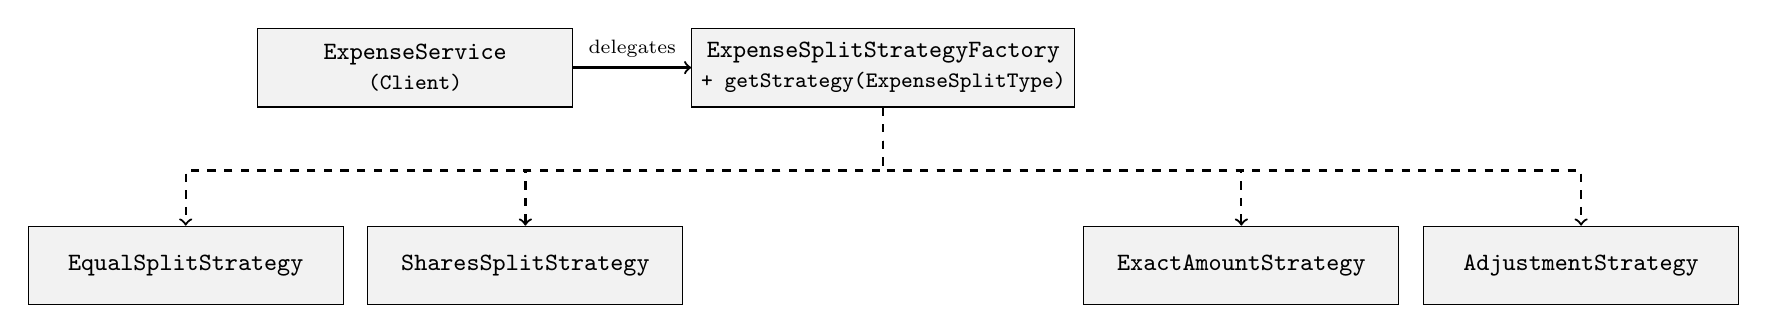
\begin{tikzpicture}[
    node distance=1.5cm and 0.3cm,
    class/.style={
        rectangle, draw=black, fill=gray!10,
        minimum width=4cm, minimum height=1cm,
        align=center, font=\small\ttfamily
    },
    uses/.style={->, thick},
    creates/.style={->, dashed, thick}
]

% 1. Factory (Center anchor point)
\node[class] (factory) {
    \textbf{ExpenseSplitStrategyFactory} \\
    \footnotesize + getStrategy(ExpenseSplitType)
};

% 2. Client (Positioned relative to the factory)
\node[class, left=1.5cm of factory] (client) {
    \textbf{ExpenseService} \\
    \footnotesize (Client)
};

% 3. Products (Positioned in a row below the factory)
\node[class, below left=1.5cm and 0.1cm of factory] (shares) {\textbf{SharesSplitStrategy}};
\node[class, left=0.3cm of shares] (equal) {\textbf{EqualSplitStrategy}};
\node[class, below right=1.5cm and 0.1cm of factory] (exact) {\textbf{ExactAmountStrategy}};
\node[class, right=0.3cm of exact] (adjust) {\textbf{AdjustmentStrategy}};

% 4. Relationships
\draw[uses] (client) -- node[above, font=\scriptsize] {delegates} (factory);

% Use orthogonal paths (-- ++(x,y) -|) for cleanly branched creation lines
% The arrows drop down 0.8cm from the factory's south anchor, then branch horizontally
\draw[creates] (factory.south) -- ++(0, -0.8) -| (equal.north);
\draw[creates] (factory.south) -- ++(0, -0.8) -| (shares.north);
\draw[creates] (factory.south) -- ++(0, -0.8) -| (exact.north);
\draw[creates] (factory.south) -- ++(0, -0.8) -| (adjust.north);

\end{tikzpicture}}%
\caption{Simple Factory Pattern: Strategy Resolution}
\end{figure}

\begin{lstlisting}[language=Java, caption=Strategy Factory Switch Expression]
public ExpenseSplitStrategy getStrategy(ExpenseSplitType splitType) {
    return switch (splitType) {
        case EQUAL_SPLIT  -> equalSplitStrategy;
        case SHARES       -> sharesSplitStrategy;
        case EXACT_AMOUNT -> exactAmountStrategy;
        case ADJUSTMENT   -> adjustmentStrategy;
    };
}
\end{lstlisting}

This centralizes the strategy-resolution logic in one place: the \texttt{ExpenseService} never needs to know which concrete class implements a given split type.

\textbf{Comparison with the standard GoF Factory pattern.}
\begin{itemize}
    \item \textbf{Simple Factory vs Factory Method:} The implementation does not follow the classic \textit{Factory Method} pattern, in which the creator is an abstraction and instantiation is delegated to subclasses. Instead, it follows the \textit{Simple Factory} idiom: a single concrete class uses conditional logic (the \texttt{switch} expression) to select among existing instances. This is a pragmatic choice appropriate to the project's scale: a full Factory Method hierarchy would introduce unnecessary abstraction layers without a tangible benefit, since the set of split types is closed (defined by an enumeration) and unlikely to grow frequently.
    \item \textbf{Instance reuse vs creation:} In the classic Factory pattern, the factory \textit{creates} new objects on each call. Our factory instead \textit{returns} pre-existing singleton beans managed by Spring's IoC container. Because the strategies are stateless, this reuse is safe and eliminates the overhead of repeated object construction.
\end{itemize}

\subsection{Debt Lifecycle and Netting Algorithm}
\label{sec:debt-lifecycle}
Debts are never created or managed directly by the user; they are a derived consequence of expenses and settlements. The \texttt{DebtService.addDebt} method implements a netting algorithm that maintains a compact and consistent debt graph across the household.

When a new debt of value $d$ is to be recorded from user A (debtor) to user B (creditor) within a household, the algorithm proceeds as follows:
\begin{enumerate}
    \item If A and B are the same user, the operation is a no-op (a user cannot owe themselves).
    \item The system checks whether an \emph{inverse} debt exists---that is, a record where B owes A in the same household. If such a record exists:
    \begin{itemize}
        \item If the inverse debt's amount is greater than $d$, the inverse debt is reduced by $d$ and the operation terminates. No forward debt is created.
        \item If the inverse debt's amount equals $d$, the two obligations cancel out perfectly. The inverse debt's amount is set to zero and the operation terminates.
        \item If the inverse debt's amount is less than $d$, the inverse debt is zeroed out and the algorithm continues with the remaining difference as the new $d$.
    \end{itemize}
    \item After netting, the system checks whether a forward debt already exists from A to B. If so, the existing amount is incremented by $d$. Otherwise, a new \texttt{Debt} entity is created with amount $d$.
\end{enumerate}

The following listing shows the core of this algorithm as implemented in the \texttt{DebtService}:

\begin{lstlisting}[language=Java, caption=Debt Netting Algorithm (Simplified)]
public void addDebt(UUID debtorId, UUID creditorId,
                    UUID householdId, BigDecimal amount) {
    if (debtorId.equals(creditorId)) return;
    BigDecimal netAmount = amount;

    // 1. Check for an inverse debt (creditor owes debtor)
    final Debt inverseDebt = debtRepository
        .findByDebtorAndCreditorAndHousehold(creditor, debtor, household)
        .orElse(null);

    if (inverseDebt != null) {
        final int cmp = inverseDebt.getAmount().compareTo(netAmount);
        if (cmp > 0) {
            // Inverse debt absorbs the new amount entirely
            inverseDebt.setAmount(inverseDebt.getAmount().subtract(netAmount));
            debtRepository.save(inverseDebt);
            return;
        } else if (cmp == 0) {
            // Perfect cancellation: zero out, do not delete
            inverseDebt.setAmount(BigDecimal.ZERO);
            debtRepository.save(inverseDebt);
            return;
        } else {
            // Partial cancellation: zero out and carry remainder
            netAmount = netAmount.subtract(inverseDebt.getAmount());
            inverseDebt.setAmount(BigDecimal.ZERO);
            debtRepository.save(inverseDebt);
        }
    }

    // 2. Increment existing forward debt or create a new one
    final Debt existingDebt = debtRepository
        .findByDebtorAndCreditorAndHousehold(debtor, creditor, household)
        .orElse(null);

    if (existingDebt != null) {
        existingDebt.setAmount(existingDebt.getAmount().add(netAmount));
        debtRepository.save(existingDebt);
    } else {
        debtRepository.save(new Debt(debtor, creditor, household, netAmount));
    }
}
\end{lstlisting}

A fundamental design decision governs the persistence of these records: when a debt's amount reaches zero---whether through settlement, netting, or exact cancellation---the entity is \emph{not} deleted from the database. Instead, the row is preserved with a zero balance. This deliberate choice avoids a wasteful cycle of destroying and recreating structurally identical entities (same debtor, same creditor, same household) whenever financial balances fluctuate due to new expenses or settlements. The zero-amount row acts as a reusable slot: should the same pair of users generate a new obligation in the same direction, the existing row is simply incremented rather than a new one being inserted. This approach guarantees a key invariant: for any ordered pair of users within a household, at most one debt record exists at any time, regardless of how many expenses have been shared between them.

\subsection{Settlement Processing}
A settlement represents a real-world payment made by a debtor to a creditor. The \texttt{SettlementService.settleDebt} method executes the following steps within a single transaction:
\begin{enumerate}
    \item The target \texttt{Debt} entity and the requesting user are fetched from the database.
    \item The system validates that the requesting user is indeed the debtor on the referenced debt, that the specified creditor matches the debt record, that the settlement amount does not exceed the current debt balance, and that the amount is strictly positive.
    \item A new \texttt{Settlement} entity is created, recording the debt reference, both parties, the amount, an optional description, and the current timestamp. The household is denormalized from the debt into the settlement for query efficiency.
    \item The debt's balance is reduced by the settlement amount. If the settlement fully covers the debt, the balance is set to exactly zero (a soft close), consistent with the zero-persistence policy described above.
\end{enumerate}

\subsection{Dynamic Query Filtering with the Specification Pattern}
\label{sec:pattern-specification}
All list-retrieval operations across the financial and chore subsystems support dynamic, composable filtering through the Specification pattern, implemented via the JPA Criteria API.

\begin{figure}[H]
\centering
\resizebox{\textwidth}{!}{%
\begin{tikzpicture}[
    class/.style={
        rectangle, draw=black, fill=gray!10,
        minimum width=4cm, minimum height=1cm,
        align=center, font=\small\ttfamily
    },
    interface/.style={
        rectangle, draw=black, fill=gray!10,
        minimum width=4cm, minimum height=1cm,
        align=center, font=\small\ttfamily
    },
    uses/.style={->, thick},
    impl/.style={->, dashed, thick}
]

% 1. Interface (Top Center)
\node[interface] (spec) at (0, 0) {
    \guillemotleft interface\guillemotright \\
    \textbf{Specification<T>} \\
    \footnotesize + toPredicate(Root, CriteriaQuery, CriteriaBuilder)
};

% 2. Implementations
% We anchor them using "north east" and "north west" to fixed coordinates.
% This guarantees their top edges align perfectly on the y-axis (-1.5),
% and creates an exact 2cm gap horizontally in the middle (-1 to 1) for the solid arrow.
\node[class, anchor=north east] (query) at (-1, -1.5) {
    \textbf{QuerySpecification} \\
    \footnotesize + buildDebtFilter(...) \\
    \footnotesize + buildExpenseFilter(...) \\
    \footnotesize + buildSettlementFilter(...)
};

\node[class, anchor=north west] (chore) at (1, -1.5) {
    \textbf{ChoreAssignmentSpecification} \\
    \footnotesize + buildAssignmentFilter(...)
};

% 3. Repository
% Placed directly in the center (x=0), safely below the bottom of the tall nodes.
\node[interface, anchor=north] (repo) at (0, -4.5) {
    \guillemotleft interface\guillemotright \\
    \textbf{JpaSpecificationExecutor<T>} \\
    \footnotesize + findAll(Specification<T>)
};

% 4. Relationships
% The dashed lines go up exactly 0.5cm (safely in the empty space),
% branch horizontally, and connect cleanly to the left and right sides of the top interface.
\draw[impl] (query.north) -- ++(0, 0.5) -| ([xshift=-2.5cm]spec.south);
\draw[impl] (chore.north) -- ++(0, 0.5) -| ([xshift=2.5cm]spec.south);

% The execution line shoots straight up the 2cm gap in the middle.
% pos=0.3 places the text lower down so it sits cleanly in the empty space.
\draw[uses] (repo.north) -- node[right, pos=0.3, font=\scriptsize] {executes} (spec.south);

\end{tikzpicture}}%
\caption{Specification Pattern: Dynamic Query Construction}
\end{figure}

\textbf{Implementation description.} Two utility classes, \texttt{QuerySpecification} (for expenses, debts, and settlements) and \texttt{ChoreAssignmentSpecification} (for chore assignments), provide static factory methods that convert filter DTOs into \texttt{Specification} lambda expressions. Each method builds a list of \texttt{Predicate} objects from the non-null fields in the filter DTO, combining them with a logical AND. The resulting specification is then passed to the repository's \texttt{findAll(Specification)} method for execution. This approach avoids writing a combinatorial number of named queries: filters for household, user role (creditor, debtor, or all), date range, and description text are composed programmatically as conjunctive predicates, and only the filters provided by the client are included in the final query.

\textbf{Comparison with the standard.}
\begin{itemize}
    \item \textbf{Domain-Driven Design origin:} The Specification pattern originates from Eric Evans' \textit{Domain-Driven Design} book, where it encapsulates a business rule as a composable, reusable object. Spring Data JPA's \texttt{Specification<T>} interface is a direct implementation of this concept, mapping the \texttt{isSatisfiedBy} method to the JPA Criteria API's \texttt{toPredicate} method.
    \item \textbf{Composability:} The standard pattern emphasizes composing specifications via logical operators (\texttt{and}, \texttt{or}, \texttt{not}). Our implementation achieves this internally by building a list of predicates and combining them with \texttt{criteriaBuilder.and()}, which is functionally equivalent. The static factory method approach was chosen over individual specification classes because the filter combinations are always conjunctive (AND-only) and do not require the full expressive power of arbitrary composition.
    \item \textbf{Avoiding query explosion:} Without this pattern, each combination of optional filters would require a separate named query method in the repository (e.g., \texttt{findByHouseholdAndDebtor}, \texttt{findByHouseholdAndCreditor}, \texttt{findByHouseholdAndDebtorAndDateRange}, etc.), leading to a combinatorial explosion. The Specification pattern reduces this to a single \texttt{findAll(Specification)} call, regardless of how many filters are active.
\end{itemize}

\section{Global Exception Management}
Uncaught application exceptions typically result in generic HTTP 500 errors and potential stack-trace leaks which formulate a security vulnerability.
The codebase utilizes a centralized exception interception mechanism, indicated by the \texttt{GlobalExceptionHandler} component. 
Through \texttt{@ControllerAdvice}, any custom thrown exception (e.g. \texttt{UserNotFoundException}) natively rewrites its response header to specific HTTP error codes (e.g. 404 Not Found), parsing the error into structured JSON output matching the \texttt{Shared} module failure payload standards.


\chapter{Frontend Design and Implementation}
\section{Presentation Layer Design}

The application's user interface is built on a single main window, in which the application's main content is only loaded after a user successfully authenticates. The entire user interface is built in a hierarchical structure, in which the main screen contains all the sub-components specific of each functionality, as the following figure shows. Each static UI component is defined with its own FXML file, the detailed explanation of the structure's functionality comes in the next chapter.

\begin{figure}[htbp]
\centering
\begin{minipage}{0.5\textwidth}
\dirtree{%
.1 resources/.
.2 popups/.
.3 assignments/.
.4 popup\_create\_assignment.fxml.
.3 expenses/.
.4 popup\_create\_expense.fxml.
.4 popup\_you\_owe.fxml.
.4 popup\_you\_are\_owed.fxml.
.4 popup\_settle\_debt.fxml.
.3 household/.
.4 popup\_create\_chore.fxml.
.4 popup\_manage\_members.fxml.
.4 popup\_invite\_member.fxml.
.4 popup\_chores\_list.fxml.
.4 popup\_shopping\_lists.fxml.
.4 popup\_list\_details.fxml.
.4 popup\_create\_household.fxml.
.3 user/.
.3 popup\_confirm.fxml.
.2 tabs/.
.3 household\_tab\_wrapper/.
.4 tab\_household.fxml.
.4 tab\_no\_household.fxml.
.3 tab\_assignments.fxml.
.3 tab\_expenses.fxml.
.3 tab\_user.fxml.
.2 auth.fxml.
.2 main.fxml.
}
\end{minipage}
\caption{Frontend FXML Structure}
\end{figure}

As the directory structure shows, the authentication screen is completely separated from the real application area, and the main file contains all of the other sub-components within it, more precisely they are loaded in a specific component of that file which will serve as the main content container. The user interface makes use of popups to display and allow interaction with the application's main functionalities. 

\begin{figure}
    \centering
    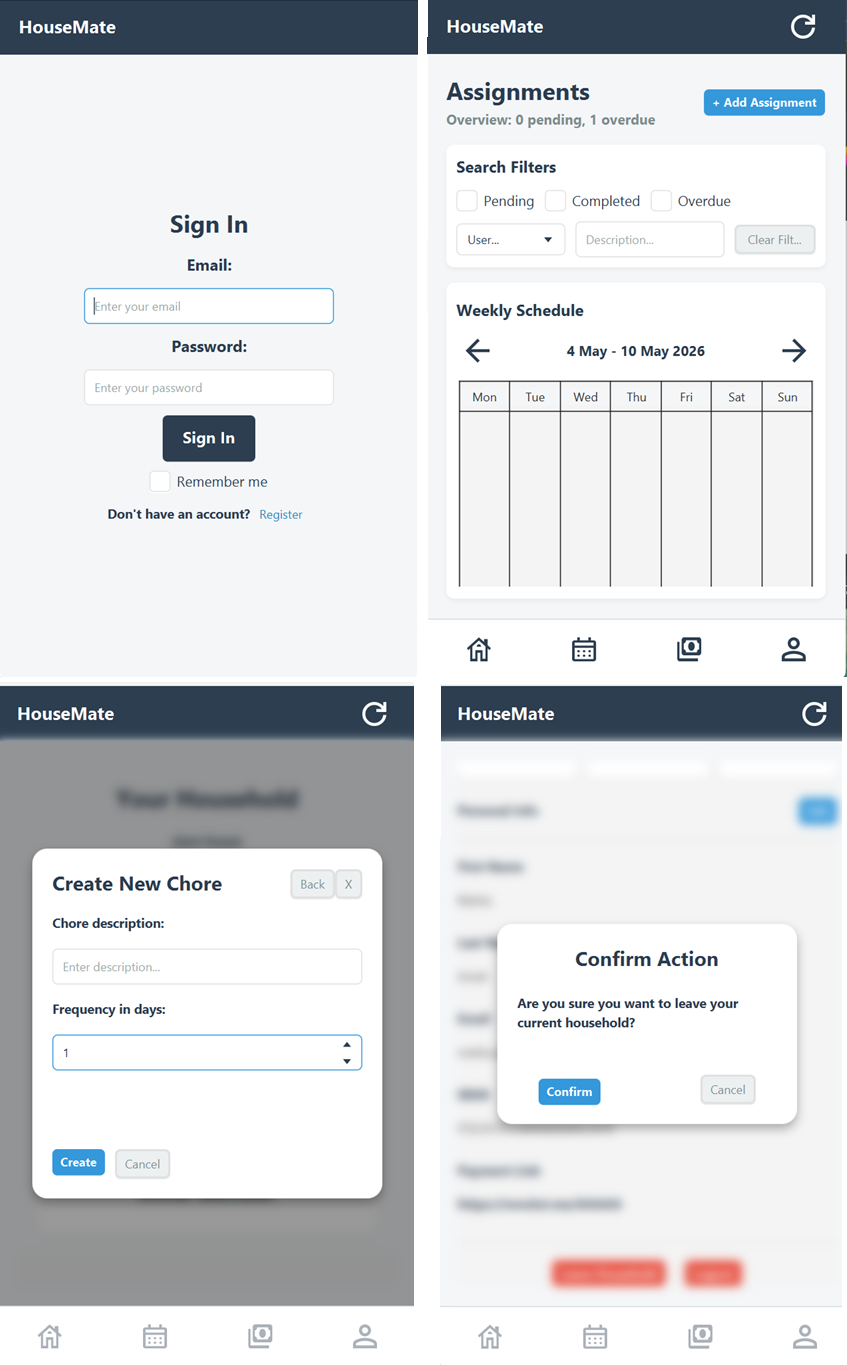
\includegraphics[width=0.8\linewidth]{images/complete_ui_screenshot..png}
    \caption{Examples of the user interface's appearance and structure}
\end{figure}

The images make clear how the authentication screen is completely separate from the rest of the client, how the main application is composed of the four tabs (Household, Assignments, Expenses, User) and how each tab contains its own popups for specific functionalities.




\section{Frontend-Backend Communication}

\subsection{Performing HTTP Requests}

The application's client module is able to communicate with the backend by performing HTTP requests to the endpoints it exposes. This responsibility is assigned to the \texttt{ClientService} classes, of which there is one for each principal domain model entity and which expose simple Java methods to the UI handling code, and act as bridges between the Java objects required by JavaFX to handle data and the JSON payloads that the backend module responds to calls with. All the client services are composed with a base helper class, \texttt{HttpRestClient}, whose responsibilities are performing that Java-JSON translation (serialization-deserialization) with the \texttt{ObjectMapper} class from the \texttt{Jackson} dependency and actually sending the HTTP request, using the native Java module \texttt{java.net.http.HttpClient} and handling all the specific exceptions that the methods of these classes can throw. Using these helper methods, the ones in the client service classes become extremely simple:
\newline
\begin{lstlisting}[language=Java, caption=Example of an HTTP request performing method in the client services (UserClientService)]
public UserResponseDTO updateCurrentUser(UserUpdateRequestDTO requestDTO) {
    String requestBody = httpRestClient.serializeDTO(requestDTO);

    HttpRequest request = HttpRequest.newBuilder()
            .uri(URI.create(BASE_URL + "/api/users/me"))
            .header("Content-Type", "application/json")
            .header("Accept", "application/json")
            .header("Authorization", httpRestClient.buildAuthHeader())
        .method("PATCH", HttpRequest.BodyPublishers.ofString(requestBody))
            .build();

    HttpResponse<String> response = httpRestClient.sendRequest(request);

    if (response.statusCode() == 200) {
        return httpRestClient.deserializeDTO(response.body(), UserResponseDTO.class);
    }

    throw new RuntimeException(
            "Failed to update current user. Server responded with status code: " + response.statusCode() + " and message: " + response.body()
    );
}
\end{lstlisting}

It is noticeable how every request includes a header with the user's JWT to authenticate itself and pass through the security layers.


\subsection{Storing Key Information}
The application is able to maintain in the client's system some useful data, to avoid clogging the server with multiple backend calls for the same purpose: this is implemented by the \texttt{SessionManager}, \texttt{AppServices}, and \texttt{JwtPersistanceHandler classes}, which respectively have the following responsibilities:
\begin{itemize}
    \item \texttt{SessionManager:} contains instances of Response DTOs related to the currently logged user, its household and its members: this data is updated when a refresh is performed, and is used on many different backend calls. Not including this would require the client to perform an additional request for almost every functionality, effectively doubling the load on the server.
    \item \texttt{AppServices:} serves as a wrapper class: it contains an instance of each different client service, as well as the SessionManager instance. This is almost required to make the injection of all the dependencies down the Controller classes possible: not using this class would add tens of lines of boilerplate code to every load of a different page.
    \item \texttt{JwtPersistanceHandler:} used to implement the "Remember Me" functionality. Since a user can authenticate itself with a valid JWT if the option to do so is chosen, this class relies on the Java native \texttt{java.util.prefs.Preferences}, which safely stores the token (received from the login endpoint) in a system registry and is able to retrieve it and attempt to use it to skip the email-and-password login step. If the token saved in the system expires or becomes no longer valid in any way, the application falls back to the standard login screen.
\end{itemize}


\section{UI/UX Functionalities}

\subsection{FXML Page Building and Loading}
The core building block of all the application's user interface are the static pages built with FXML files. These files consist of a composition of JavaFX components, which can generally be referred to as nodes, nested into each other to allow the construction of organized and well-defined layouts. Here follows, as an example, part of the main page's code:\clearpage

\begin{lstlisting}[language=XML, caption=Core structure of the client's main window]
<BorderPane prefHeight="750.0" prefWidth="420.0" styleClass="root" xmlns="http://javafx.com/javafx/21" xmlns:fx="http://javafx.com/fxml/1" fx:controller="com.housemate.client.controllers.MainController">
    <top>
        <!--Logo and "Refresh" button-->
    </top>

    <center>
        <StackPane fx:id="outerContainer">
            <StackPane fx:id="mainContentContainer"/>
            <StackPane fx:id="popupLayer" mouseTransparent="true"/>
            <StackPane fx:id = "confirmPopupLayer" mouseTransparent="true"/>
        </StackPane>
    </center>

    <bottom>
        <HBox alignment="CENTER" prefHeight="60.0" styleClass="nav-bar" BorderPane.alignment="CENTER">
            <Button fx:id="btnNavH" maxWidth="Infinity" prefHeight="60.0" styleClass="nav-button-active" HBox.hgrow="ALWAYS">
                <graphic>
                    <Region styleClass="base-icon, household-nav-button"/>
                </graphic>
            </Button>
            <!--Three more exactly equal buttons for the other tabs-->
        </HBox>
    </bottom>

</BorderPane>
\end{lstlisting}

As the first statement of the example shows, each file is linked to its own Controller Java class with the \texttt{fx:controller} attribute within the root node. These classes are responsible for handling the interactions between the user and the interface elements, performing calls to the client services and visualizing incoming data from the backend.
\newline

The Controller hierarchy is exactly the same as the fxml files one, since they are in a 1:1 relationship.

\begin{lstlisting}[language=Java, caption=Code to load a FXML file (from the MainController class)]
FXMLLoader loaderAssignments = new FXMLLoader(getClass().getResource("/com/housemate/client/tabs/tab_assignments.fxml"));
loaderAssignments.setControllerFactory(clazz -> new TabAssignmentsController(this.services, this));
tabAssignments = loaderAssignments.load();
tabAssignmentsController = loaderAssignments.getController();
\end{lstlisting}

All the loaders have to use the \texttt{setControllerFactory} method to allow the injection of the \texttt{AppServices} and other required dependencies to the corresponding Controllers.

\subsection{Hierarchical Structure of the Controllers}

\begin{figure}[H]
\centering
\begin{minipage}{0.5\textwidth}
\dirtree{%
.1 controllers/.
.2 AuthScreenController.java.
.2 MainController.java/.
.3 PopupConfirmActionController.java.
.3 HouseholdTabWrapperController.java/.
.4 TabHouseholdController.java/.
.5 PopupChoresList.java.
.5 PopupCreateChoreController.java.
.5 PopupCreateListController.java.
.5 PopupInviteMemberController.java.
.5 PopupListDetailsController.java.
.5 PopupManageMembersController.java.
.5 PopupShoppingListsController.java.
.4 TabNoHouseholdController.java/.
.5 PopupCreateHouseholdController.java.
.5 PopupJoinHouseholdController.java.
.3 TabAssignmentsController.java/.
.4 PopupCreateAssignmentsController.java.
.3 TabExpensesController.java/.
.4 PopupCreateExpenseController.java.
.4 PopupSettleDebtController.java.
.4 PopupYouAreOwedController.java.
.4 PopupYouOweController.java.
}
\end{minipage}
\caption{Complete structure of the Controller hierarchy}
\end{figure}

As the previous code snippet and the structure diagram showed, when the \texttt{MainController} loads the FXML files relative to the four main application tabs, it passes itself (\texttt{this}) down to their Controllers. This has been repeated in the following steps, such that the tabs Controllers pass down the \texttt{MainController} reference to those of the popups they load. This structure has been chosen to allow the main controller to be the only responsible for showing graphical elements to the user: whenever any Controller wants a popup to be opened, a different tab to be displayed or a success/error message to be displayed, all they have to do is call the \texttt{MainController}'s corresponding methods.

This implementation allows for both paths of the hierarchy to be taken: when a button within a tab is clicked, the corresponding controller can call both the \texttt{MainController} to open a popup and call the popup's controller itself to perform some actions, which is usually the backend call to fetch the information specific to that popup. 

\subsection{Application Launch}
All JavaFX applications are required to have their entry point defined by a class which extends \texttt{javafx.Application}. The main method of the program has to call the static method \texttt{Application.launch()}: JavaFX then automatically calls the \texttt{start} method, which has to be overridden in the entry point class. Here is part of HouseMate's client launcher class:
\clearpage

\begin{lstlisting}[language=Java, caption=Structure of the client module's entry point]

public class HouseMateApplication extends Application {

    private final HttpClient httpClient = HttpClient.newHttpClient();
    private final ObjectMapper objectMapper = new ObjectMapper().registerModule(new JavaTimeModule());
    private final SessionManager clientContext = new SessionManager(new AuthState());

    private AppServices services;
    private Stage primaryStage;

    @Override
    public void start(Stage primaryStage) {

        this.primaryStage = primaryStage;
        this.services = new AppServices(httpClient, objectMapper, clientContext);

        //retrieve session data and validate it
       //call to either showLoginScreen or showMainScreen depending on the saved session
    }

    public void logout(){
        //clear session 
        showLoginScreen();
    }

    public void showLoginScreen() {
        //load FXML
        primaryStage.show();
    }

    public void showMainScreen() {
        //load FXML
        primaryStage.show();
    }
}

    
\end{lstlisting}

This method is also the only place in the applications which instantiates the AppServices, HttpClient, ObjectMapper and SessionManager dependencies and injects them down the Controller hierarchy by applying the controller factory technique on the MainController

\subsection{Dynamic UI Components Loading}

\subsection{Performing Backend Calls}

Through the entire client module development, the fundamental rule of JavaFX had to be followed: \textit{"Every action that interacts with JavaFX UI components must be performed on the JavaFX Application Thread"}. The JavaFX Application Thread is the main thread of every application build this way and all code runs by default on it. Because of that, if a backend call were to be performed within such thread and the code had to wait for the response (which can take a perceivable amount of time, depending on server latency and connection), the entire UI would be frozen until the response comes back because no UI-updating code could be executed. The necessary workaround consists of encapsulating the client service methods into a separate thread, with the native Java \texttt{CompletableFuture} module. When running any Java program, the JVW keeps a pool of background threads available for use. The static method \texttt{CompletableFuture.runAsync(() -> {})} executes the provided \texttt{Runnable} on one of these threads. Running the backend calls with this construct allows for the UI to be responsive while waiting for a response from the backend. \newline
\begin{lstlisting}[language=Java, caption=Core procedure required to perform a backend call]
ChoreCreateRequestDTO requestDTO = new ChoreCreateRequestDTO(
    txtChoreDesc.getText(),
    spnFrequencyDays.getValue(),
    services.getSessionManager().getCurrentHousehold().id()
);

CompletableFuture.runAsync(() -> {
    try {
        services.getChoreClientService().createChore(requestDTO);
        Platform.runLater(() -> {
            clearFields();
            mainController.showToast("Chore created successfully!", MessageType.SUCCESS);
            onReturnCallback.run();
        });
    } catch (RuntimeException e) {
        Platform.runLater(() -> mainController.showToast(e.getMessage(), MessageType.ERROR));
    }
});
\end{lstlisting}

This snippet also shows the creation of the request DTO inside the Controller classes, which read the information provided by the user on the UI components (whenever more complex information is required to perform an action, such as expense creation, the data is not directly read from the JavaFX components but passed through temporary private variables) and perform the actual HTTP request by opportunely calling the client services. This enforces the separation of responsibilities applied to the project. Since all the code inside the \texttt{CompletableFuture} block is executed on a separate thread, the UI-updating code has to be run back on the JavaFX Application Thread, with its \texttt{Platform.runLater(() -> {})} which simply executes the provided Runnable after the separate thread it's invoked in terminates.

\section{Frontend Design Patterns}
\label{sec:frontend-patterns}

\subsection{Fa\c{c}ade Pattern}

\begin{figure}[H]
\centering
\resizebox{\textwidth}{!}{%
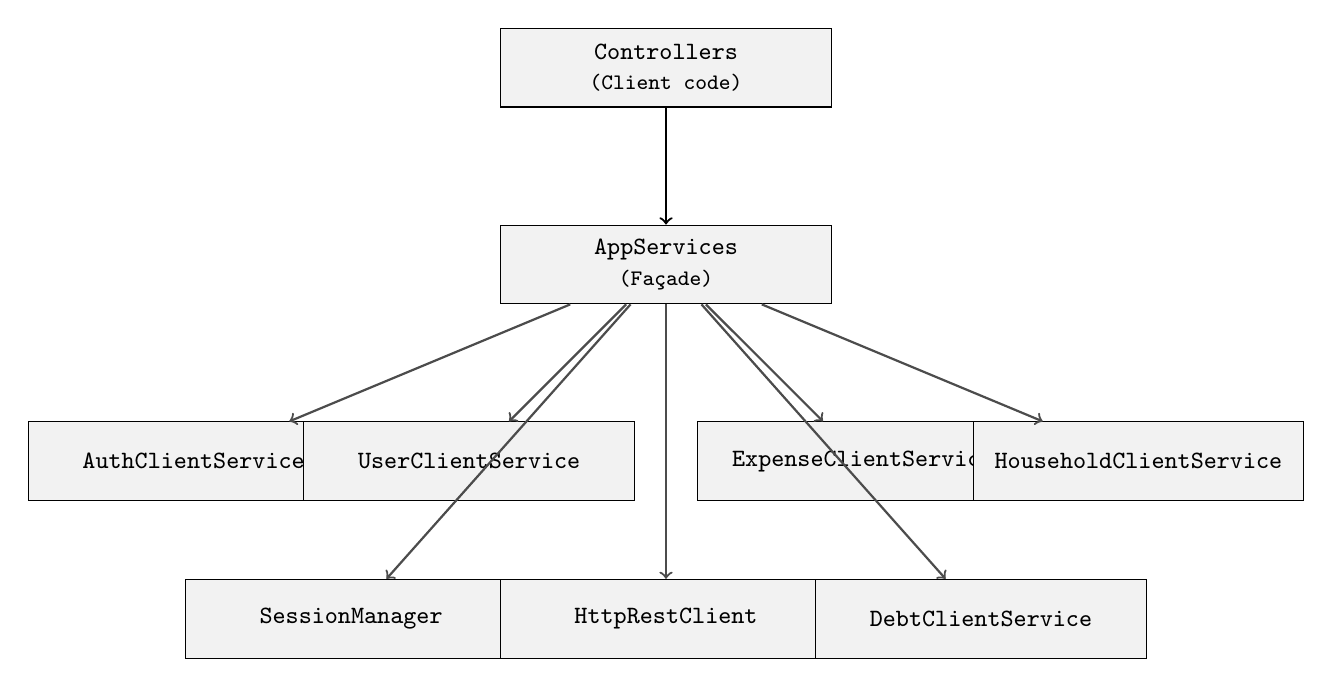
\begin{tikzpicture}[
    class/.style={
        rectangle, draw=black, fill=gray!10,
        minimum width=4.2cm, minimum height=1cm,
        align=center, font=\small\ttfamily
    },
    uses/.style={->, thick},
    contains/.style={->, thick, draw=black!70}
]

% Facade
\node[class] (facade) at (0, 3) {
    \textbf{AppServices} \\
    \footnotesize (Fa\c{c}ade)
};

% Subsystem services
\node[class] (auth) at (-6, 0.5) {\textbf{AuthClientService}};
\node[class] (user) at (-2.5, 0.5) {\textbf{UserClientService}};
\node[class] (expense) at (2.5, 0.5) {\textbf{ExpenseClientService}};
\node[class] (household) at (6, 0.5) {\textbf{HouseholdClientService}};
\node[class] (session) at (-4, -1.5) {\textbf{SessionManager}};
\node[class] (http) at (0, -1.5) {\textbf{HttpRestClient}};
\node[class] (debt) at (4, -1.5) {\textbf{DebtClientService}};

% Client
\node[class] (client) at (0, 5.5) {
    \textbf{Controllers} \\
    \footnotesize (Client code)
};

% Relationships
\draw[uses] (client) -- (facade);
\draw[contains] (facade) -- (auth);
\draw[contains] (facade) -- (user);
\draw[contains] (facade) -- (expense);
\draw[contains] (facade) -- (household);
\draw[contains] (facade) -- (session);
\draw[contains] (facade) -- (http);
\draw[contains] (facade) -- (debt);

\end{tikzpicture}}%
\caption{Fa\c{c}ade Pattern: Unified Service Access}
\end{figure}

\textbf{Implementation description.} The \texttt{AppServices} class acts as a Fa\c{c}ade over the entire client-side service subsystem. It aggregates instances of all eight client services (\texttt{AuthClientService}, \texttt{UserClientService}, \texttt{HouseholdClientService}, \texttt{ChoreClientService}, \texttt{ExpenseClientService}, \texttt{DebtClientService}, \texttt{SettlementClientService}, \texttt{ShoppingListClientService}), the \texttt{SessionManager}, and the underlying \texttt{HttpRestClient}. Controllers never instantiate or manage service dependencies themselves; they receive a single \texttt{AppServices} reference during FXML loading and use its getters to access any service they need.

\textbf{Comparison with the standard.}
\begin{itemize}
    \item \textbf{Simplified interface:} The GoF Fa\c{c}ade pattern provides a unified, simplified interface to a complex subsystem. \texttt{AppServices} fulfills this precisely: without it, every controller would need to receive and manage references to eight independent services plus the session manager, resulting in extensive boilerplate code in each controller's constructor.
    \item \textbf{Not hiding the subsystem:} In the strict GoF definition, the Fa\c{c}ade can optionally hide the subsystem classes entirely, exposing only high-level methods. Our implementation exposes the individual services through getters (e.g., \texttt{getExpenseClientService()}) rather than wrapping their methods. This is a deliberate trade-off: wrapping every method of every service would create a monolithic class with dozens of delegating methods, contradicting the Single Responsibility Principle, while still providing no additional abstraction.
\end{itemize}

\subsection{Mediator Pattern}

\begin{figure}[H]
\centering
\resizebox{\textwidth}{!}{%
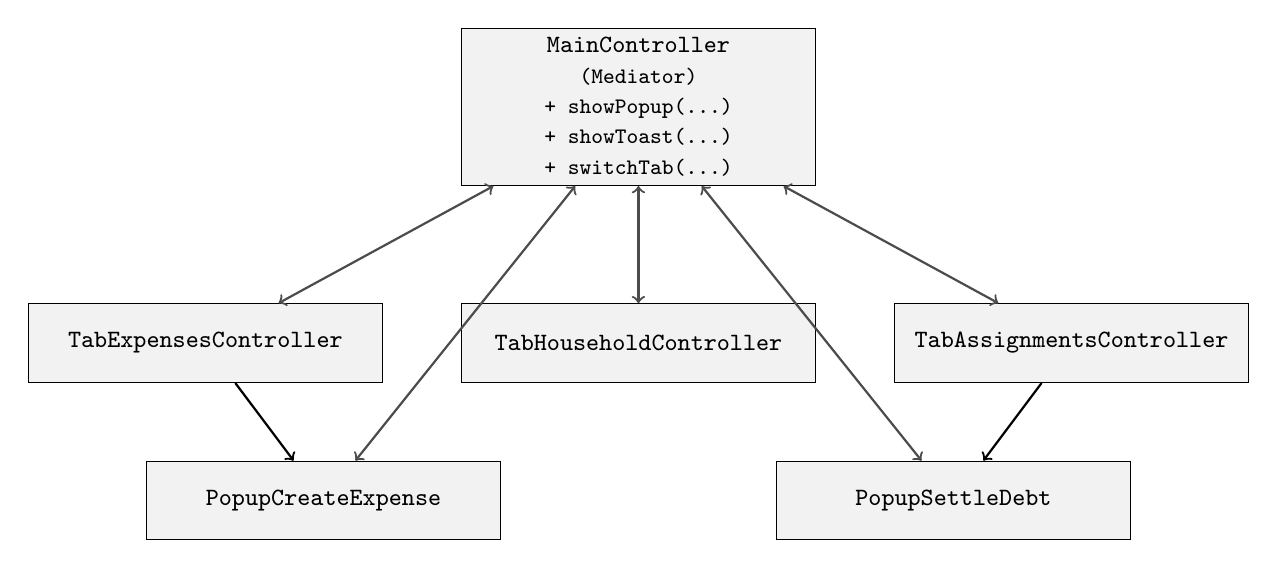
\begin{tikzpicture}[
    class/.style={
        rectangle, draw=black, fill=gray!10,
        minimum width=4.5cm, minimum height=1cm,
        align=center, font=\small\ttfamily
    },
    mediates/.style={<->, thick, draw=black!70},
    calls/.style={->, thick}
]

% Mediator
\node[class] (mediator) at (0, 3) {
    \textbf{MainController} \\
    \footnotesize (Mediator) \\
    \footnotesize + showPopup(...) \\
    \footnotesize + showToast(...) \\
    \footnotesize + switchTab(...)
};

% Colleagues
\node[class] (tab1) at (-5.5, 0) {\textbf{TabExpensesController}};
\node[class] (tab2) at (0, 0) {\textbf{TabHouseholdController}};
\node[class] (tab3) at (5.5, 0) {\textbf{TabAssignmentsController}};
\node[class] (popup1) at (-4, -2) {\textbf{PopupCreateExpense}};
\node[class] (popup2) at (4, -2) {\textbf{PopupSettleDebt}};

% Relationships
\draw[mediates] (tab1) -- (mediator);
\draw[mediates] (tab2) -- (mediator);
\draw[mediates] (tab3) -- (mediator);
\draw[calls] (tab1) -- (popup1);
\draw[calls] (tab3) -- (popup2);
\draw[mediates] (popup1) -- (mediator);
\draw[mediates] (popup2) -- (mediator);

\end{tikzpicture}}%
\caption{Mediator Pattern: Centralized UI Coordination}
\end{figure}

\textbf{Implementation description.} The \texttt{MainController} acts as a central Mediator for all user interface coordination in the JavaFX client. When the FXML hierarchy is loaded, every child controller (tabs and popups) receives a reference to the \texttt{MainController} via the \texttt{setControllerFactory} mechanism. Whenever a child controller needs to open a popup, display a success or error toast, or trigger a tab switch, it calls a method on the \texttt{MainController} (e.g., \texttt{showPopup}, \texttt{showToast}). No child controller ever communicates directly with another child controller; all cross-component interactions are routed through the mediator.

\textbf{Comparison with the standard.}
\begin{itemize}
    \item \textbf{Concrete vs Abstract Mediator:} The GoF pattern defines the Mediator as an interface or abstract class, allowing multiple mediator implementations. Our application uses a single concrete \texttt{MainController} because the JavaFX client has exactly one main window with one coordination point. Introducing an abstract mediator would add unnecessary complexity without a realistic use case for substitution.
    \item \textbf{Bidirectional communication:} In the standard pattern, colleagues notify the mediator of events, and the mediator decides how to respond. Our implementation follows this closely: child controllers call the mediator's methods (upward direction), and the mediator manipulates the shared \texttt{StackPane} layers to display popups and toasts (downward direction). The child controllers never directly access the \texttt{popupLayer} or \texttt{confirmPopupLayer} nodes.
    \item \textbf{Decoupling benefit:} Without this mediator, each of the 15+ controllers would need references to every other controller it might interact with, creating a tightly coupled mesh of dependencies. The mediator reduces this to a star topology where each controller knows only the \texttt{MainController}.
\end{itemize}



\chapter{Testing and Quality Assurance}
\section{Testing Philosophy and Approach}
In an application with the described articulated structure, software correctness cannot be inferred from visual inspection alone: security flaws or financial inaccuracies are categories of defects that remain invisible during development but can produce serious consequences in production, thus they must be prevented. To this end, a test-driven verification strategy was adopted. Every business-critical component is accompanied by automated tests that exercise happy-path behavior, validate edge cases, and ensure that invalid or adversarial inputs get rejected.

The structure of this testing landscape follows the \emph{Test Pyramid} model, as described below:
\begin{enumerate}[itemsep=4pt, parsep=0pt]
    \item \textbf{Unit Tests (Base Tier):} A broad base of fast, isolated tests that verify individual classes and methods;
    \item \textbf{Repository Tests (Middle Tier):} A repository layer that exercises persistence against a real, in-memory database;
    \item \textbf{Web-Layer Tests (Top Tier):} A specialized suite that validates HTTP semantics, authentication enforcement, and JSON contract compliance.
\end{enumerate}
This layered approach ensures that smaller defects are caught as early and as cheaply as possible in the unit tests, while the integration tests guarantee that the application architecture remains stable at runtime.

\section{Testing Technology Stack}

\begin{table}[H]
\centering
\renewcommand{\arraystretch}{1.2}
\begin{tabular}{@{}lp{10cm}@{}}
\toprule
\textbf{Technology} & \textbf{Description and Role in the Test Suite} \\ \midrule
JUnit 5 & The unit testing framework that allows to write and execute the tests, while also providing useful annotations such as \texttt{@Test}, \texttt{@Nested}, \texttt{@BeforeEach}, and \texttt{@DisplayName}, all widely used throughout the testing codebase. \\
Mockito & A mocking library used to create lightweight stubs of any component and infrastructure dependency in order to isolate the unit under test from external state. \\
AssertJ & An assertion library; preferred over JUnit's built-in assertions for its improved readability and strong support for \texttt{BigDecimal} comparison semantics, mainly needed to test the expense management module (see section \ref{sec:core-expense_management}). \\
Spring Boot Test & Provides the \texttt{@WebMvcTest} and \texttt{@DataJpaTest} test slices for controller and repository test classes. The benefit is that these annotations instruct the system to bootstrap only the Spring context layers required by the involved tests, minimizing startup and overall testing times. \\
Spring Security Test & Supplies the \texttt{@WithMockUser}, \texttt{@WithAnonymousUser}, and \texttt{csrf()} utilities used to simulate authenticated and unauthenticated HTTP requests in controller tests. \\
MockMvc & Spring's HTTP test client, which dispatches requests through the full DispatcherServlet pipeline (filters, serialization, exception handling) without starting a real web server. \\
H2 Database & Lightweight in-memory relational database that mirrors the PostgreSQL schema via Hibernate's \texttt{create-drop} DDL mode, providing a fresh state for every test execution. \\
TestEntityManager & \textit{Spring Data JPA} utility that wraps the JPA \texttt{EntityManager}, offering \texttt{persistAndFlush} and \texttt{clear} methods for precise control over the persistence context in integration tests. \\
\bottomrule
\end{tabular}
\caption{Testing technology stack}
\label{tab:test-stack}
\end{table}


\section{Unit Testing}
To illustrate the concrete application of our testing methodology, this section walks through specific unit test examples across the entire application stack. We will begin with basic function testing and gradually move up through the various tiers of the web architecture. Additionally, a dedicated subsection covers security testing, highlighting how unit tests can prevent vulnerabilities and enforce access control policies at the code level.

% \subsection{Domain Model Validation Tests}
% The domain entity constructors perform eager input validation: null references, non-positive monetary amounts, and missing descriptions are rejected before any persistence operation is attempted. The model test classes exercise these guard clauses exhaustively.

% \begin{lstlisting}[language=Java, caption=Representative model validation tests (ExpenseTest)]
% @Nested
% class ConstructorTests {

%     @Test
%     void constructor_withValidArguments_createsExpense() {
%         Expense expense = new Expense(
%                 "Groceries",
%                 new BigDecimal("50.00"),
%                 payer, household,
%                 ExpenseSplitType.EQUAL_SPLIT
%         );
%         assertThat(expense.getDescription()).isEqualTo("Groceries");
%         assertThat(expense.getAmount()).isEqualByComparingTo("50.00");
%         assertThat(expense.getDate()).isNotNull();
%     }

%     @Test
%     void constructor_nullAmount_throwsIllegalArgumentException() {
%         assertThatThrownBy(() -> new Expense(
%                 "Groceries", null, payer, household,
%                 ExpenseSplitType.EQUAL_SPLIT))
%                 .isInstanceOf(IllegalArgumentException.class)
%                 .hasMessageContaining("Expense amount cannot be null");
%     }

%     @Test
%     void constructor_negativeAmount_throwsIllegalArgumentException() {
%         assertThatThrownBy(() -> new Expense(
%                 "Groceries", new BigDecimal("-50.00"),
%                 payer, household, ExpenseSplitType.EQUAL_SPLIT))
%                 .isInstanceOf(IllegalArgumentException.class)
%                 .hasMessageContaining("must be strictly greater than zero");
%     }
% }
% \end{lstlisting}

% Four test classes---\texttt{DebtTest}, \texttt{ExpenseTest}, \texttt{ExpenseShareTest}, and \texttt{SettlementTest}---collectively verify that every entity constructor rejects null fields, enforces positivity constraints on monetary values, and correctly initializes timestamps and empty child collections.

\subsection{Pure Function Tests (Expense Split Strategies)}
In the codebase, a perfect example of pure functions is identified by the expense splitting strategies. In fact, they receive two parameters (the total amount and the list of share requests) and return a deterministic map of user / share amount without holding any state. This makes them ideal candidates for exhaustive unit testing without any mocking. As an example, we present below one of the unit tests for the \texttt{EQUAL\_SPLIT} strategy:

\begin{lstlisting}[language=Java, basicstyle=\scriptsize\ttfamily, caption=Example of a unit test for the Equal Split Strategy]
@Test
void calculateShares_withThreeUsersAndRemainder_distributesSinglePenny() {
    Map<UUID, BigDecimal> result = strategy.calculateShares(
            new BigDecimal("10.00"),
            List.of(
                    new ExpenseShareRequestDTO(u1, null),
                    new ExpenseShareRequestDTO(u2, null),
                    new ExpenseShareRequestDTO(u3, null)
            )
    );

    assertThat(result).hasSize(3);
    assertThat(sum(result)).isEqualByComparingTo("10.00");
    assertThat(result.values()).containsExactlyInAnyOrder(
            new BigDecimal("3.34"),
            new BigDecimal("3.33"),
            new BigDecimal("3.33")
    );
}
\end{lstlisting}

While these constructs might appear straightforward to handle, actually they are the ones that need more in-depth analysis as they present a large number of edge cases and are the foundation on which the upper layers rely on.\\
In fact, sticking to the example, a critical property verified by every strategy test is the \emph{sum invariant}: the sum of all computed shares must equal the original total exactly; this assertion catches rounding errors that would otherwise accumulate silently across hundreds of transactions. The strategies are also tested for rejection of edge cases such as duplicate user IDs, null amounts, empty share lists, zero amounts, and negative amounts.

\subsection{Service Layer Tests (Adding a Debt)}
The backend service layer contains the most critical business logic, including the debt netting algorithm and the expense creation orchestration. These business logics are tested with Mockito-based unit tests that stub the repository layer, allowing the tests to run independently from the actual existence of a database. In the following snippet we provide the code of a unit test for the debt addition logic:

\begin{lstlisting}[language=Java, basicstyle=\scriptsize\ttfamily, caption=Example of a unit test for the Debt Service]
@Test
void addDebt_whenInverseDebtMatchesExactly_setsInverseDebtToZero() {
    BigDecimal amount = new BigDecimal("50.00");
    when(userRepository.findById(debtorId))
            .thenReturn(Optional.of(debtor));
    when(userRepository.findById(creditorId))
            .thenReturn(Optional.of(creditor));
    when(householdRepository.findById(householdId))
            .thenReturn(Optional.of(household));

    Debt inverseDebt = mock(Debt.class);
    when(inverseDebt.getAmount()).thenReturn(amount);
    when(debtRepository
            .findByDebtorAndCreditorAndHousehold(creditor, debtor, household))
            .thenReturn(Optional.of(inverseDebt));

    debtService.addDebt(debtorId, creditorId, householdId, amount);

    verify(inverseDebt).setAmount(BigDecimal.ZERO);
    verify(debtRepository).save(inverseDebt);
    verifyNoMoreInteractions(debtRepository);
}
\end{lstlisting}

The \texttt{DebtServiceTest} class uses Mockito's \texttt{ArgumentCaptor} extensively to inspect the exact entities passed to \texttt{debtRepository.save()}, verifying not only that the correct method was called but that the saved entity carries the expected amount, debtor, creditor, and household. The test suite covers all five branches of the netting algorithm:
\begin{enumerate}
    \item Debtor equals creditor (short-circuit, no repository calls).
    \item No inverse debt exists: a new forward debt is created.
    \item Inverse debt is greater than the new amount: inverse debt is reduced.
    \item Inverse debt equals the new amount exactly: inverse debt is set to zero.
    \item Inverse debt is smaller than the new amount: inverse debt is zeroed, and a forward debt is created for the remainder.
\end{enumerate}

Each service test class also tests guard clauses: null user IDs, null filter DTOs, missing entities (user not found, household not found), and unauthorized state transitions (e.g. attempting to view debts without an active household membership). These tests use AssertJ's \texttt{assertThatThrownBy} to verify both the exception type and the error message.

\subsection{Controller Layer Tests (Creating an Expense)}
Controller tests use Spring's \texttt{@WebMvcTest} test slice, which bootstraps only the web layer and the security filter chain, while mocking all service dependencies. This approach verifies that endpoints:
\begin{itemize}
    \item Return the correct HTTP status codes for success (e.g. 200 \texttt{OK}, 201 \texttt{CREATED}) and failure (e.g. 400 \texttt{BAD REQUEST}, 401 \texttt{UNAUTHORIZED}, 403 \texttt{FORBIDDEN});
    \item Serialize response DTOs to the expected JSON structure;
    \item Reject invalid request payloads before they reach the service layer;
    \item Enforce authentication (via \texttt{@WithAnonymousUser}) and authorization correctly.
\end{itemize}

In the following example we provide a unit test for expense creation that handles both success and failure cases, ensuring the controller returns the correct status code in each situation and follows the correct behaviour both in terms of returned results and accessed services.
\begin{lstlisting}[language=Java, basicstyle=\scriptsize\ttfamily, caption=Example of a unit test for the Expense Controller]
@WebMvcTest(ExpenseController.class)
@ContextConfiguration(classes = ServerApp.class)
@WithMockUser(username = "11111111-1111-1111-1111-111111111111")
class ExpenseControllerTest {

    @Test
    @DisplayName("POST /api/expenses - returns 201 with created expense")
    void testCreateExpense_Success() throws Exception {
        when(expenseService.createExpense(eq(TEST_USER_UUID), any()))
                .thenReturn(expenseResponse);

        mockMvc.perform(post(BASE_URL)
                    .with(csrf())
                    .contentType("application/json")
                    .content(objectMapper.writeValueAsString(validCreateRequest)))
                .andExpect(status().isCreated())
                .andExpect(jsonPath("$.id").value(EXPENSE_ID))
                .andExpect(jsonPath("$.description").value("Groceries"))
                .andExpect(jsonPath("$.amount")
                        .value(comparesEqualTo(
                            new BigDecimal("120.00")), BigDecimal.class
                        ))
                .andExpect(jsonPath("$.splitType")
                        .value(ExpenseSplitType.EQUAL_SPLIT.name()));

        verify(expenseService).createExpense(eq(TEST_USER_UUID), any());
    }

    @Test
    @WithAnonymousUser
    @DisplayName("POST /api/expenses - returns 401 for unauthenticated user")
    void testCreateExpense_Unauthenticated() throws Exception {
        mockMvc.perform(post(BASE_URL).with(csrf())
                        .contentType("application/json")
                        .content(objectMapper.writeValueAsString(
                            validCreateRequest
                        )))
                .andExpect(status().isUnauthorized());

        verify(expenseService, never()).createExpense(any(), any());
    }
}
\end{lstlisting}

The use of \texttt{@WithMockUser} and \texttt{@WithAnonymousUser} annotations allows the test suite to verify the entire Spring Security filter chain end-to-end, including the \texttt{JwtAuthenticationFilter}, without constructing actual JWT tokens. The \texttt{csrf()} processor is applied to all state-changing requests to comply with Spring Security's CSRF protection.

\subsection{Client Service Tests}
Each \texttt{ClientService} test class mocks the \texttt{HttpRestClient} helper to simulate DTOs serialization, JSON deserialization and server responses, then verifies that:
\begin{enumerate}
    \item HTTP requests are constructed with the correct method, URI path, query parameters, content type, and \texttt{Authorization} header.
    \item Successful responses (status 2xx) are correctly deserialized into the expected DTO types.
    \item Error responses produce a \texttt{RuntimeException} containing the expected status code and server message.

\end{enumerate}

\begin{lstlisting}[language=Java, basicstyle=\scriptsize\ttfamily, caption=Example of a unit test for the Expense Client Service]
@Test
@DisplayName("createExpense - should successfully create an expense")
void testCreateExpense_Success() throws Exception {
    String jsonResponse = objectMapper.writeValueAsString(testExpenseResponseDTO);
    HttpResponse<String> mockResponse = createMockResponse(201, jsonResponse);

    when(mockHttpRestClient.serializeDTO(any())).thenReturn("{\"description\":\"Groceries\"}");
    when(mockHttpRestClient.sendRequest(any(HttpRequest.class)))
            .thenReturn(mockResponse);
    when(mockHttpRestClient.deserializeDTO(
                jsonResponse, ExpenseResponseDTO.class
            )
        )
            .thenReturn(testExpenseResponseDTO);
    when(mockHttpRestClient.buildAuthHeader())
            .thenReturn("Bearer test-token");

    ExpenseResponseDTO result = expenseClientService
            .createExpense(testExpenseCreateRequestDTO);

    assertNotNull(result);
    assertEquals(TEST_EXPENSE_ID, result.id());
    assertEquals(TEST_DESCRIPTION, result.description());

    verify(mockHttpRestClient).serializeDTO(any());
    ArgumentCaptor<HttpRequest> requestCaptor = ArgumentCaptor.forClass(
        HttpRequest.class
    );
    verify(mockHttpRestClient).sendRequest(requestCaptor.capture());
    verify(mockHttpRestClient).deserializeDTO(
        jsonResponse, ExpenseResponseDTO.class
    );
    verify(mockHttpRestClient).buildAuthHeader();

    HttpRequest capturedRequest = requestCaptor.getValue();
    assertEquals("POST", capturedRequest.method());
    assertTrue(capturedRequest.uri().getPath().endsWith("/api/expenses"));
    assertEquals("application/json", capturedRequest.headers()
        .firstValue("Content-Type").orElse(null)
    );
    assertEquals("Bearer test-token", capturedRequest.headers()
        .firstValue("Authorization").orElse(null)
    );
}
\end{lstlisting}

The use of \texttt{ArgumentCaptor} on the \texttt{HttpRequest} object is a key technique: it allows the test to inspect the exact URI, HTTP method, headers, and content type of the request that the service would send to the real server, guaranteeing that the client and server agree on the API contract.

\subsection{Security Layer Tests}
Given the sensitivity of authentication mechanisms, the security filters require dedicated unit tests to guarantee that invalid, expired, or missing credentials are appropriately managed without degrading into server errors. The \texttt{JwtAuthenticationFilterTest} achieves this by isolating the filtering logic from the web application utilizing \texttt{MockHttpServletRequest}, \texttt{MockHttpServletResponse}, and \texttt{MockFilterChain}.

By mocking the underlying \texttt{JwtService} and \texttt{UserService}, the test suite systematically simulates various edge cases. These include requests with no \texttt{Authorization} header, tokens with an invalid UUID format, and tokens triggering exceptions. A critical requirement verified by these tests is that token parsing errors (such as \texttt{ExpiredJwtException} or \texttt{MalformedJwtException}) do not propagate as internal server errors (HTTP 500). Instead, the filter safely aborts the authentication process while allowing the filter chain to continue, gracefully delegating the rejection logic to the downstream security components:

\begin{lstlisting}[language=Java, basicstyle=\scriptsize\ttfamily, caption=Example of a unit test verifying expired token handling in the JWT Filter]
@Test
void expiredToken_jwtExceptionCaught_filterPassesThrough_noAuthentication() throws Exception {
    String token = "expired.jwt.token";
    MockHttpServletRequest request = new MockHttpServletRequest();
    request.addHeader("Authorization", "Bearer " + token);
    MockHttpServletResponse response = new MockHttpServletResponse();
    MockFilterChain chain = new MockFilterChain();

    when(jwtService.extractSubject(token))
            .thenThrow(new ExpiredJwtException(null, null, "Token expired"));

    jwtAuthenticationFilter.doFilterInternal(request, response, chain);

    assertThat(SecurityContextHolder.getContext().getAuthentication()).isNull();
    assertThat(response.getStatus()).isEqualTo(200); // Filter chain continues downstream without crashing
}
\end{lstlisting}

This approach guarantees that the security context (\texttt{SecurityContextHolder}) is only populated upon successful validation of a legitimate token, effectively securing the application state right at the entry point of the filter chain.

\subsection{Global Exception Handler Tests}
To ensure that business logic constraints and unexpected errors are consistently translated into robust HTTP responses, the application uses a centralized \texttt{@RestControllerAdvice}. The \texttt{GlobalExceptionHandlerTest} suite verifies this component by directly invoking its handler methods with various mocked or instantiated exceptions.

These unit tests confirm that specific exception types map to the correct HTTP status codes and payload formats as described in section \ref{sec:global-exception-handler}. Notably, a strong emphasis is placed on ensuring complex validation errors, which throw \texttt{BindException}, are handled reliably. The tests guarantee that the handler correctly extracts multiple field errors, aggregates them into a structured key-value map, and gracefully falls back to default messages such as \texttt{"Invalid value"} when specific error text is missing:

\begin{lstlisting}[language=Java, basicstyle=\scriptsize\ttfamily, caption=Example of a unit test for validation error handling]
@Test
void handleValidationExceptions_methodArgumentNotValid_multipleErrors() {
    MethodArgumentNotValidException exception = mock(
        MethodArgumentNotValidException.class
    );
    BindingResult bindingResult = mock(BindingResult.class);
    List<ObjectError> errors = new ArrayList<>();
    errors.add(new FieldError("objectName", "email", "Invalid email format"));
    errors.add(new FieldError(
            "objectName", "password", "Password must be at least 8 characters"
        )
    );
    errors.add(new FieldError("objectName", "name", "Name cannot be blank"));

    when(exception.getBindingResult()).thenReturn(bindingResult);
    when(bindingResult.getAllErrors()).thenReturn(errors);

    ResponseEntity<Map<String, String>> response = 
            globalExceptionHandler.handleValidationExceptions(exception);

    assertThat(response.getStatusCode()).isEqualTo(HttpStatus.BAD_REQUEST);
    assertThat(response.getBody())
            .containsEntry("error", "Validation Failed")
            .containsEntry("email", "Invalid email format")
            .containsEntry("password", "Password must be at least 8 characters")
            .containsEntry("name", "Name cannot be blank");
}
\end{lstlisting}

This comprehensive verification guards against internal stack traces leaking to the client layer and enforces a predictable, client-friendly error reporting contract across the application's REST APIs.



\section{Integration Testing}

While unit tests verify individual components in isolation, integration tests verify that multiple layers collaborate correctly when wired together by the Spring context. Three integration test classes use the \texttt{@DataJpaTest} slice combined with \texttt{@Import} to load the real service classes alongside an H2 in-memory database, while mocking only the components that are not relevant to the test scenario.

\subsection{Expense Creation Integration Test}
The \texttt{ExpenseServiceIntegrationTest} verifies the full transactional flow of expense creation: persisting the expense entity, creating the expense shares, and generating the corresponding debt records. The test persists real \texttt{User}, \texttt{Household}, and \texttt{HouseholdMembership} entities via the \texttt{TestEntityManager}, then invokes \texttt{expenseService.createExpense} and asserts that the database contains the expected expense shares and debt rows.

\begin{lstlisting}[language=Java, caption=Verifying the full expense creation transaction (ExpenseServiceIntegrationTest)]
@Test
@DisplayName("createExpense persists expense graph and creates debt rows")
void createExpense_persistsExpenseAndCreatesDebtsForNonPayerShares() {
    Household household = persistHousehold("Main Household");
    User payer = persistUser("Alice", "Payer", "alice@test.com");
    User debtor = persistUser("Bob", "Debtor", "bob@test.com");
    persistMembership(household, payer, true);
    persistMembership(household, debtor, false);

    // ... strategy mock configuration ...

    ExpenseResponseDTO result = expenseService.createExpense(
            payer.getId(), request);

    assertThat(result.id()).isNotNull();
    assertThat(result.shares()).hasSize(2);
    assertThat(debtRepository.findAll())
        .hasSize(1)
        .first()
        .satisfies(savedDebt -> {
            assertThat(savedDebt.getDebtor().getId()).isEqualTo(debtor.getId());
            assertThat(savedDebt.getCreditor().getId()).isEqualTo(payer.getId());
            assertThat(savedDebt.getAmount()).isEqualByComparingTo("20.00");
        });
}
\end{lstlisting}

\subsection{Debt Netting Integration Test}
The \texttt{DebtServiceIntegrationTest} exercises the netting algorithm against a real H2 database, verifying three critical scenarios:
\begin{enumerate}
    \item When a new debt is smaller than an existing inverse debt, the inverse debt is reduced and no new row is created.
    \item When a new debt exceeds an existing inverse debt, the inverse debt is set to zero and a forward remainder is created as a separate row.
    \item When a new debt exactly cancels an existing inverse debt, the inverse debt's amount is set to zero and the row is preserved (not deleted), confirming the zero-persistence design decision described in the backend chapter.
\end{enumerate}

\subsection{Settlement Integration Test}
The \texttt{SettlementServiceIntegrationTest} verifies that settling a debt correctly persists the \texttt{Settlement} entity and reduces the \texttt{Debt} balance within a single transaction. Two scenarios are tested: a partial settlement that reduces the debt from 100.00 to 60.00, and a full settlement that sets the debt to exactly zero without deleting the debt row.


\section{Complete Test Inventory}

The following table provides a complete inventory of all test classes in the codebase, organized by module and architectural layer. The two modules, \texttt{backend} and \texttt{client}, are presented separately.

\begin{longtable}{@{}p{3.5cm}p{6.5cm}p{3cm}@{}}
\toprule
\textbf{Layer} & \textbf{Test Class} & \textbf{Test Type} \\ \midrule
\endfirsthead

\toprule
\textbf{Layer} & \textbf{Test Class} & \textbf{Test Type} \\ \midrule
\endhead

\midrule \multicolumn{3}{r}{\textit{Continued on next page}} \\
\endfoot

\bottomrule
\endlastfoot

\multicolumn{3}{@{}l}{\cellcolor{UCRow}\textbf{Backend Module}} \\[2pt]

Config / Security
    & \texttt{GlobalExceptionHandlerTest}
    & Unit \\
    & \texttt{JwtAuthenticationFilterTest}
    & Unit \\[4pt]

Controller
    & \texttt{AuthControllerTest}
    & Web Slice \\
    & \texttt{ChoreControllerTest}
    & Web Slice \\
    & \texttt{DebtControllerTest}
    & Web Slice \\
    & \texttt{ExpenseControllerTest}
    & Web Slice \\
    & \texttt{HouseholdControllerTest}
    & Web Slice \\
    & \texttt{SettlementControllerTest}
    & Web Slice \\
    & \texttt{ShoppingListControllerTest}
    & Web Slice \\
    & \texttt{UserControllerTest}
    & Web Slice \\[4pt]

Repository
    & \texttt{ChoreAssignmentRepositoryTest}
    & Data Slice \\
    & \texttt{DebtRepositoryTest}
    & Data Slice \\
    & \texttt{DebtSpecificationTest}
    & Data Slice \\
    & \texttt{ExpenseRepositoryTest}
    & Data Slice \\
    & \texttt{ExpenseSpecificationTest}
    & Data Slice \\
    & \texttt{HouseholdRepositoryTest}
    & Data Slice \\
    & \texttt{QuerySpecificationTest}
    & Data Slice \\
    & \texttt{SettlementRepositoryTest}
    & Data Slice \\
    & \texttt{SettlementSpecificationTest}
    & Data Slice \\
    & \texttt{UserRepositoryTest}
    & Data Slice \\[4pt]

Service
    & \texttt{AuthServiceTest}
    & Unit \\
    & \texttt{ChoreServiceTest}
    & Unit \\
    & \texttt{DebtServiceTest}
    & Unit \\
    & \texttt{ExpenseServiceTest}
    & Unit \\
    & \texttt{HouseholdServiceTest}
    & Unit \\
    & \texttt{JwtServiceTest}
    & Unit \\
    & \texttt{SettlementServiceTest}
    & Unit \\
    & \texttt{ShoppingListServiceTest}
    & Unit \\
    & \texttt{UserServiceTest}
    & Unit \\[4pt]

Strategy
    & \texttt{AdjustmentStrategyTest}
    & Unit \\
    & \texttt{EqualSplitStrategyTest}
    & Unit \\
    & \texttt{ExactAmountStrategyTest}
    & Unit \\
    & \texttt{ExpenseSplitStrategyFactoryTest}
    & Unit \\
    & \texttt{SharesSplitStrategyTest}
    & Unit \\[4pt]

Integration
    & \texttt{DebtServiceIntegrationTest}
    & Integration \\
    & \texttt{ExpenseServiceIntegrationTest}
    & Integration \\
    & \texttt{SettlementServiceIntegrationTest}
    & Integration \\[8pt]

\multicolumn{3}{@{}l}{\cellcolor{UCRow}\textbf{Client Module}} \\[2pt]

Client Service
    & \texttt{AuthClientServiceTest}
    & Unit \\
    & \texttt{ChoreClientServiceTest}
    & Unit \\
    & \texttt{DebtClientServiceTest}
    & Unit \\
    & \texttt{ExpenseClientServiceTest}
    & Unit \\
    & \texttt{HouseholdClientServiceTest}
    & Unit \\
    & \texttt{HttpRestClientTest}
    & Unit \\
    & \texttt{SettlementClientServiceTest}
    & Unit \\
    & \texttt{ShoppingListClientServiceTest}
    & Unit \\
    & \texttt{UserClientServiceTest}
    & Unit \\

\end{longtable}

In total, the test suite comprises \textbf{48 test classes} spanning 6 architectural layers across 2 modules. The backend module accounts for 39 test classes and the client module contributes 9 test classes, each mirroring a corresponding client service.

\section{Test Environment Configuration}

The test environment is isolated from production through a dedicated Spring profile. The \texttt{application-test.properties} file configures:

\begin{lstlisting}[caption=Test environment configuration]
jwt.secret=<TEST_PROFILE_JWT_SECRET>
jwt.expiration-ms=86400000

# H2 in-memory database
spring.jpa.hibernate.ddl-auto=create-drop
\end{lstlisting}

The \texttt{create-drop} DDL strategy guarantees that Hibernate generates the complete schema from the entity annotations at startup and destroys it at shutdown, providing a clean database for every test execution. The H2 dependency is scoped to \texttt{runtime} in the backend's \texttt{pom.xml}, ensuring it is available during testing but excluded from the production deployment artifact, where PostgreSQL is used instead.

The \texttt{@DataJpaTest} annotation activates this configuration automatically for repository and integration tests, providing:
\begin{itemize}
    \item Automatic rollback after each test method, preventing state leakage between tests.
    \item A \texttt{TestEntityManager} bean for fine-grained control over entity persistence and cache clearing.
    \item Exclusion of non-JPA Spring components (web controllers, security filters, etc.), keeping the test context minimal and fast.
\end{itemize}

\chapter{Project Management and Conclusion}
\section{Project Summary}
The HouseMate project proved to be a substantive undertaking that solidified concepts embedded deeply within complex software engineering. We transitioned from initial requirement elicitations all the way through physical deployment, maintaining rigorous methodologies surrounding database schema creation, client-server REST paradigms, and security enforcement.

Automating chore tracking, household finances, and shared coordination reduces cognitive overhead for residents and tackles a real-world friction point efficiently. By building separate and highly decoupled Java components (a Spring Boot backend, a Java client, and shared DTOs), we ensured robust extensibility.

\section{Challenges and Learnings}
Several challenges were encountered and appropriately solved during the execution phase:
\begin{enumerate}
    \item \textbf{Object-Relational Mapping (ORM) Complexities:} Translating arbitrary financial debts connecting User instances across an arbitrary Expense record proved to be challenging due to circular relational logic constraints. Breaking this down via specific bridging tables (\texttt{ExpenseShare}) established necessary clarity.
    \item \textbf{Authentication Logistics:} Passing context implicitly throughout the web-filter chains leveraging JWTs required comprehensive thread-safe considerations in Spring contexts. Understanding the \texttt{SecurityContextHolder} allowed for proper authorization strategies.
    \item \textbf{Dependency Scope Isolations:} Utilizing a multi-modules Maven project required understanding exactly which libraries must trace dependencies backwards into the \texttt{Shared} module without creating circular dependencies.
\end{enumerate}

\section{Future Work}
Although the application achieves all MVP (Minimum Viable Product) objectives, logical extensions for scaling the ecosystem include:
\begin{itemize}
    \item \textbf{Mobile Application Support:} Since the Backend is completely separated from the Frontend, integrating a Kotlin (Android) or Swift (iOS) client requires zero backend logic changes, opening the ecosystem up completely to portable devices.
    \item \textbf{Push Notifications:} Alerting household members asynchronously when new debts originate or when chores are overdue via WebSockets or Firebase Integration.
    \item \textbf{Payment Gateway Integrations:} Facilitating absolute real-world financial settlement integrations via Stripe APIs or PayPal architectures instead of relying solely on tracking internal ledger variables.
\end{itemize}


\end{document}